% Generated by Sphinx.
\def\sphinxdocclass{report}
\documentclass[letterpaper,10pt,openany,oneside]{sphinxmanual}
\usepackage[utf8]{inputenc}
\DeclareUnicodeCharacter{00A0}{\nobreakspace}
\usepackage[T1]{fontenc}
\usepackage[english]{babel}
\usepackage{times}
\usepackage[Bjarne]{fncychap}
\usepackage{longtable}
\usepackage{sphinx}
\usepackage{multirow}


\title{Pandemic Exemplar with OpenMP}
\date{March 11, 2014}
\release{}
\author{CSinParallel Project}
\newcommand{\sphinxlogo}{}
\renewcommand{\releasename}{}
\makeindex

\makeatletter
\def\PYG@reset{\let\PYG@it=\relax \let\PYG@bf=\relax%
    \let\PYG@ul=\relax \let\PYG@tc=\relax%
    \let\PYG@bc=\relax \let\PYG@ff=\relax}
\def\PYG@tok#1{\csname PYG@tok@#1\endcsname}
\def\PYG@toks#1+{\ifx\relax#1\empty\else%
    \PYG@tok{#1}\expandafter\PYG@toks\fi}
\def\PYG@do#1{\PYG@bc{\PYG@tc{\PYG@ul{%
    \PYG@it{\PYG@bf{\PYG@ff{#1}}}}}}}
\def\PYG#1#2{\PYG@reset\PYG@toks#1+\relax+\PYG@do{#2}}

\expandafter\def\csname PYG@tok@gd\endcsname{\def\PYG@tc##1{\textcolor[rgb]{0.63,0.00,0.00}{##1}}}
\expandafter\def\csname PYG@tok@gu\endcsname{\let\PYG@bf=\textbf\def\PYG@tc##1{\textcolor[rgb]{0.50,0.00,0.50}{##1}}}
\expandafter\def\csname PYG@tok@gt\endcsname{\def\PYG@tc##1{\textcolor[rgb]{0.00,0.25,0.82}{##1}}}
\expandafter\def\csname PYG@tok@gs\endcsname{\let\PYG@bf=\textbf}
\expandafter\def\csname PYG@tok@gr\endcsname{\def\PYG@tc##1{\textcolor[rgb]{1.00,0.00,0.00}{##1}}}
\expandafter\def\csname PYG@tok@cm\endcsname{\let\PYG@it=\textit\def\PYG@tc##1{\textcolor[rgb]{0.25,0.50,0.56}{##1}}}
\expandafter\def\csname PYG@tok@vg\endcsname{\def\PYG@tc##1{\textcolor[rgb]{0.73,0.38,0.84}{##1}}}
\expandafter\def\csname PYG@tok@m\endcsname{\def\PYG@tc##1{\textcolor[rgb]{0.13,0.50,0.31}{##1}}}
\expandafter\def\csname PYG@tok@mh\endcsname{\def\PYG@tc##1{\textcolor[rgb]{0.13,0.50,0.31}{##1}}}
\expandafter\def\csname PYG@tok@cs\endcsname{\def\PYG@tc##1{\textcolor[rgb]{0.25,0.50,0.56}{##1}}\def\PYG@bc##1{\setlength{\fboxsep}{0pt}\colorbox[rgb]{1.00,0.94,0.94}{\strut ##1}}}
\expandafter\def\csname PYG@tok@ge\endcsname{\let\PYG@it=\textit}
\expandafter\def\csname PYG@tok@vc\endcsname{\def\PYG@tc##1{\textcolor[rgb]{0.73,0.38,0.84}{##1}}}
\expandafter\def\csname PYG@tok@il\endcsname{\def\PYG@tc##1{\textcolor[rgb]{0.13,0.50,0.31}{##1}}}
\expandafter\def\csname PYG@tok@go\endcsname{\def\PYG@tc##1{\textcolor[rgb]{0.19,0.19,0.19}{##1}}}
\expandafter\def\csname PYG@tok@cp\endcsname{\def\PYG@tc##1{\textcolor[rgb]{0.00,0.44,0.13}{##1}}}
\expandafter\def\csname PYG@tok@gi\endcsname{\def\PYG@tc##1{\textcolor[rgb]{0.00,0.63,0.00}{##1}}}
\expandafter\def\csname PYG@tok@gh\endcsname{\let\PYG@bf=\textbf\def\PYG@tc##1{\textcolor[rgb]{0.00,0.00,0.50}{##1}}}
\expandafter\def\csname PYG@tok@ni\endcsname{\let\PYG@bf=\textbf\def\PYG@tc##1{\textcolor[rgb]{0.84,0.33,0.22}{##1}}}
\expandafter\def\csname PYG@tok@nl\endcsname{\let\PYG@bf=\textbf\def\PYG@tc##1{\textcolor[rgb]{0.00,0.13,0.44}{##1}}}
\expandafter\def\csname PYG@tok@nn\endcsname{\let\PYG@bf=\textbf\def\PYG@tc##1{\textcolor[rgb]{0.05,0.52,0.71}{##1}}}
\expandafter\def\csname PYG@tok@no\endcsname{\def\PYG@tc##1{\textcolor[rgb]{0.38,0.68,0.84}{##1}}}
\expandafter\def\csname PYG@tok@na\endcsname{\def\PYG@tc##1{\textcolor[rgb]{0.25,0.44,0.63}{##1}}}
\expandafter\def\csname PYG@tok@nb\endcsname{\def\PYG@tc##1{\textcolor[rgb]{0.00,0.44,0.13}{##1}}}
\expandafter\def\csname PYG@tok@nc\endcsname{\let\PYG@bf=\textbf\def\PYG@tc##1{\textcolor[rgb]{0.05,0.52,0.71}{##1}}}
\expandafter\def\csname PYG@tok@nd\endcsname{\let\PYG@bf=\textbf\def\PYG@tc##1{\textcolor[rgb]{0.33,0.33,0.33}{##1}}}
\expandafter\def\csname PYG@tok@ne\endcsname{\def\PYG@tc##1{\textcolor[rgb]{0.00,0.44,0.13}{##1}}}
\expandafter\def\csname PYG@tok@nf\endcsname{\def\PYG@tc##1{\textcolor[rgb]{0.02,0.16,0.49}{##1}}}
\expandafter\def\csname PYG@tok@si\endcsname{\let\PYG@it=\textit\def\PYG@tc##1{\textcolor[rgb]{0.44,0.63,0.82}{##1}}}
\expandafter\def\csname PYG@tok@s2\endcsname{\def\PYG@tc##1{\textcolor[rgb]{0.25,0.44,0.63}{##1}}}
\expandafter\def\csname PYG@tok@vi\endcsname{\def\PYG@tc##1{\textcolor[rgb]{0.73,0.38,0.84}{##1}}}
\expandafter\def\csname PYG@tok@nt\endcsname{\let\PYG@bf=\textbf\def\PYG@tc##1{\textcolor[rgb]{0.02,0.16,0.45}{##1}}}
\expandafter\def\csname PYG@tok@nv\endcsname{\def\PYG@tc##1{\textcolor[rgb]{0.73,0.38,0.84}{##1}}}
\expandafter\def\csname PYG@tok@s1\endcsname{\def\PYG@tc##1{\textcolor[rgb]{0.25,0.44,0.63}{##1}}}
\expandafter\def\csname PYG@tok@gp\endcsname{\let\PYG@bf=\textbf\def\PYG@tc##1{\textcolor[rgb]{0.78,0.36,0.04}{##1}}}
\expandafter\def\csname PYG@tok@sh\endcsname{\def\PYG@tc##1{\textcolor[rgb]{0.25,0.44,0.63}{##1}}}
\expandafter\def\csname PYG@tok@ow\endcsname{\let\PYG@bf=\textbf\def\PYG@tc##1{\textcolor[rgb]{0.00,0.44,0.13}{##1}}}
\expandafter\def\csname PYG@tok@sx\endcsname{\def\PYG@tc##1{\textcolor[rgb]{0.78,0.36,0.04}{##1}}}
\expandafter\def\csname PYG@tok@bp\endcsname{\def\PYG@tc##1{\textcolor[rgb]{0.00,0.44,0.13}{##1}}}
\expandafter\def\csname PYG@tok@c1\endcsname{\let\PYG@it=\textit\def\PYG@tc##1{\textcolor[rgb]{0.25,0.50,0.56}{##1}}}
\expandafter\def\csname PYG@tok@kc\endcsname{\let\PYG@bf=\textbf\def\PYG@tc##1{\textcolor[rgb]{0.00,0.44,0.13}{##1}}}
\expandafter\def\csname PYG@tok@c\endcsname{\let\PYG@it=\textit\def\PYG@tc##1{\textcolor[rgb]{0.25,0.50,0.56}{##1}}}
\expandafter\def\csname PYG@tok@mf\endcsname{\def\PYG@tc##1{\textcolor[rgb]{0.13,0.50,0.31}{##1}}}
\expandafter\def\csname PYG@tok@err\endcsname{\def\PYG@bc##1{\setlength{\fboxsep}{0pt}\fcolorbox[rgb]{1.00,0.00,0.00}{1,1,1}{\strut ##1}}}
\expandafter\def\csname PYG@tok@kd\endcsname{\let\PYG@bf=\textbf\def\PYG@tc##1{\textcolor[rgb]{0.00,0.44,0.13}{##1}}}
\expandafter\def\csname PYG@tok@ss\endcsname{\def\PYG@tc##1{\textcolor[rgb]{0.32,0.47,0.09}{##1}}}
\expandafter\def\csname PYG@tok@sr\endcsname{\def\PYG@tc##1{\textcolor[rgb]{0.14,0.33,0.53}{##1}}}
\expandafter\def\csname PYG@tok@mo\endcsname{\def\PYG@tc##1{\textcolor[rgb]{0.13,0.50,0.31}{##1}}}
\expandafter\def\csname PYG@tok@mi\endcsname{\def\PYG@tc##1{\textcolor[rgb]{0.13,0.50,0.31}{##1}}}
\expandafter\def\csname PYG@tok@kn\endcsname{\let\PYG@bf=\textbf\def\PYG@tc##1{\textcolor[rgb]{0.00,0.44,0.13}{##1}}}
\expandafter\def\csname PYG@tok@o\endcsname{\def\PYG@tc##1{\textcolor[rgb]{0.40,0.40,0.40}{##1}}}
\expandafter\def\csname PYG@tok@kr\endcsname{\let\PYG@bf=\textbf\def\PYG@tc##1{\textcolor[rgb]{0.00,0.44,0.13}{##1}}}
\expandafter\def\csname PYG@tok@s\endcsname{\def\PYG@tc##1{\textcolor[rgb]{0.25,0.44,0.63}{##1}}}
\expandafter\def\csname PYG@tok@kp\endcsname{\def\PYG@tc##1{\textcolor[rgb]{0.00,0.44,0.13}{##1}}}
\expandafter\def\csname PYG@tok@w\endcsname{\def\PYG@tc##1{\textcolor[rgb]{0.73,0.73,0.73}{##1}}}
\expandafter\def\csname PYG@tok@kt\endcsname{\def\PYG@tc##1{\textcolor[rgb]{0.56,0.13,0.00}{##1}}}
\expandafter\def\csname PYG@tok@sc\endcsname{\def\PYG@tc##1{\textcolor[rgb]{0.25,0.44,0.63}{##1}}}
\expandafter\def\csname PYG@tok@sb\endcsname{\def\PYG@tc##1{\textcolor[rgb]{0.25,0.44,0.63}{##1}}}
\expandafter\def\csname PYG@tok@k\endcsname{\let\PYG@bf=\textbf\def\PYG@tc##1{\textcolor[rgb]{0.00,0.44,0.13}{##1}}}
\expandafter\def\csname PYG@tok@se\endcsname{\let\PYG@bf=\textbf\def\PYG@tc##1{\textcolor[rgb]{0.25,0.44,0.63}{##1}}}
\expandafter\def\csname PYG@tok@sd\endcsname{\let\PYG@it=\textit\def\PYG@tc##1{\textcolor[rgb]{0.25,0.44,0.63}{##1}}}

\def\PYGZbs{\char`\\}
\def\PYGZus{\char`\_}
\def\PYGZob{\char`\{}
\def\PYGZcb{\char`\}}
\def\PYGZca{\char`\^}
\def\PYGZam{\char`\&}
\def\PYGZlt{\char`\<}
\def\PYGZgt{\char`\>}
\def\PYGZsh{\char`\#}
\def\PYGZpc{\char`\%}
\def\PYGZdl{\char`\$}
\def\PYGZti{\char`\~}
% for compatibility with earlier versions
\def\PYGZat{@}
\def\PYGZlb{[}
\def\PYGZrb{]}
\makeatother

\begin{document}

\maketitle
\tableofcontents
\phantomsection\label{index::doc}


This example contains a fully functional simulation of the type of modeling done by epidemiologists to answer the question: what happens when an infectious disease hits a population?  Code for an original serial version is provided and described in detail.  Next, descriptions of a parallel version using OpenMP is provided, where the code is modified from the original serial version.

\textbf{Acknowledgment}: Many thanks to Aaron Weeden of the Shodor Foundation for the original version of this material and code.


\chapter{Infectious Disease}
\label{0-Introduction/introduction:pandemic-modeling-exemplar-using-openmp}\label{0-Introduction/introduction:infectious-disease}\label{0-Introduction/introduction::doc}
\textbf{By Aaron Weeden, Shodor Education Foundation, Inc.} \footnote{
For original documentation and code developed by Aaron Weeden, please go to original \href{http://www.shodor.org/petascale/materials/UPModules/infectiousDisease/}{pandemic}.
}

\textbf{Heavily modified by Yu Zhao, Macalester College}

\textbf{Overview}

Epidemiology is the study of infectious disease. Infectious diseases are
said to be “contagious” among people if they are transmittable from one
person to another. Epidemiologists can use models to assist them in
predicting the behavior of infectious diseases. This module will develop
a simple agent-based infectious disease model, develop a parallel
algorithm based on the model, provide a coded implementation for the
algorithm, and explore the scaling of the coded implementation on high
performance cluster resources.

\textbf{Pre-assessment Rubric}

This rubric is to gauge students’ initial knowledge and experience with
the materials presented in this module. Students can be asked to rate their
knowledge and experience on the following scale and in the following
subject areas:
\begin{quote}

\textbf{Scale}
\begin{enumerate}
\item {} 
no knowledge, no experience

\item {} 
very little knowledge, very little experience

\item {} 
some knowledge, some experience

\item {} 
a good amount of knowledge, a good amount of experience

\item {} 
high level of knowledge, high level of experience

\end{enumerate}

\textbf{Subject areas}
\begin{itemize}
\item {} 
Disease modeling

\item {} 
Parallel Algorithm Design

\item {} 
Parallel Hardware

\item {} 
OpenMP programming

\item {} 
CUDA programming

\item {} 
Scaling parallel code

\end{itemize}
\end{quote}

Each of these topics is mentioned to some degree in the material that follows. Some familiarity with each of these is assumed, except that the disease modeling is explained here.


\section{Model}
\label{0-Introduction/introduction:model}
The model makes certain assumptions about the spread of the disease. In
particular, it assumes that the disease spreads from one person to
another person with some “contagiousness factor”, that is, some percent
chance that the disease will be transmitted. The model further assumes
that diseases can only be spread from a person who is carrying the
disease, a so-called “infected” person, to a person who is capable of
becoming infected, also known as a “susceptible” person. The disease is
assumed to have a certain incubation period, or “duration” – a length of
time during which the disease remains in the person. The disease is also
assumed to be transmittable only within a certain distance, or
“infection radius”, from a person capable of transmitting the disease.
The model further assumes that each person moves randomly at most 1 unit
in a given direction each day. Finally, the model assumes that after the
duration of the disease within a person, the person can become either
“immune” to the disease, incapable of being further infected or of
infecting other people but still able to move around, or “dead”,
incapable of being further infected, infecting other people, or moving.

The description below explains the various entities in the model. Things
in underlines are entities, things in \textbf{bold} are attributes of the
entities, and things in \emph{italics} refer to entities found elsewhere in
the description.


\includegraphics{img-0.png} (pl. people)
\begin{itemize}
\item {} 
Has a certain \textbf{X location} and a certain \textbf{Y location}, which tell where it is in the \emph{environment}.

\item {} 
Has a certain \textbf{state}, which can be either ‘susceptible’, ‘infected’, ‘immune’, or ‘dead’. States are stored in the memories of \emph{processes} and \emph{threads}. They can also be represented by color (black for susceptible, red for infected, green for immune, no color for dead), or by a ASCII character (o for susceptible, X for infected, I for immune, no character for dead).

\end{itemize}


\includegraphics{img-1.png} \emph{Disease}
\begin{itemize}
\item {} 
Has a certain \textbf{duration}, which is the number of days in which a \emph{person} remains infected.

\item {} 
Has a certain \textbf{contagiousness factor}, which is the likelihood of it spreading from one \emph{person} to another.

\item {} 
Has a certain \textbf{deadliness factor}, which is the likelihood that a \emph{person} will die from the disease. 100 minus this is the likelihood that a \emph{person} will become immune to the disease.

\end{itemize}

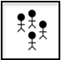
\includegraphics{img-2.png} Environment
\begin{itemize}
\item {} 
Has a certain \textbf{width} and \textbf{height}, which bound the area in which \emph{people} are able to move.

\end{itemize}


\includegraphics{img-3.png} Timer
\begin{itemize}
\item {} 
Counts the \textbf{number of days} that have elapsed in the simulation.

\end{itemize}


\includegraphics{img-4.png} Thread (pl. threads)
\begin{itemize}
\item {} 
A computational entity that controls people and performs computations.

\item {} 
Shares \textbf{memory} with other threads, a space into which threads can read and write data.

\end{itemize}


\includegraphics{img-5.png} Process (pl. processes)
\begin{itemize}
\item {} 
A computational entity that controls people and performs computations.

\item {} 
Has its own private \textbf{memory}, which is a space into which it can read and write data.

\item {} 
Has a certain \textbf{rank}, which identifies it.

\item {} 
Communicates with other processes by \textbf{passing messages}, in which it sends certain data.

\item {} 
Can spawn threads to do work for it.

\item {} 
Keeps count of how many susceptible, infected, immune, and \emph{dead} people exist.

\end{itemize}


\section{Introduction to Parallelism}
\label{0-Introduction/introduction:introduction-to-parallelism}
In parallel processing, rather than having a single program execute
tasks in a sequence, the program is split among multiple “execution
flows” executing tasks in parallel, i.e. at the same time. The term
“execution flow” refers to a discrete computational entity that performs
processes autonomously. A common synonym is “execution context”; “flow”
is chosen here because it evokes the stream of instructions that each
entity processes.

Execution flows have more specific names depending on the flavor of
parallelism being utilized. In “distributed memory” parallelism, in
which execution flows keep their own private memories (separate from the
memories of other execution flows), execution flows are known as
“processes”. In order for one process to access the memory of another
process, the data must be communicated, commonly by a technique known as
“message passing”. The standard of message passing considered in this
module is defined by the “Message Passing Interface (MPI)”, which
defines a set of primitives for packaging up data and sending them
between processes.

In another flavor of parallelism known as “shared memory”, in which
execution flows share a memory space among them, the execution flows are
known as “threads”. Threads are able to read and write to and from
memory without having to send messages. \footnote{
It should be noted that shared memory is really just a form of fast message passing. Threads must communicate, just as processes must, but threads get to communicate at bus speeds (using the front-side bus that connects the CPU to memory), whereas processes must communicate at network speeds (Ethernet, infiniband, etc.), which are much slower.
} The standard for shared
memory considered in this module is OpenMP, which uses a series of
“pragma”s, or directives for specifying parallel regions of code to be
executed by threads. \footnote{
Threads can also have their own private memories, and OpenMP has pragmas to define whether variables are public or private.
}

A third flavor of parallelism is known as “hybrid”, in which both
distributed and shared memory are utilized. In hybrid parallelism, the
problem is broken into tasks that each process executes in parallel; the
tasks are then broken further into subtasks that each of the threads
execute in parallel. After the threads have executed their sub-tasks,
the processes use the shared memory to gather the results from the
threads, use message passing to gather the results from other processes,
and then move on to the next tasks.

\textbf{Parallel Hardware}

In order to use parallelism, the underlying hardware needs to support
it. The classic model of the computer, first established by John von
Neumann in the 20:math:\emph{\{\}\textasciicircum{}\{th\}} century, has a single CPU connected to
memory. Such an architecture does not support parallelism because there
is only one CPU to run a stream of instructions. In order for
parallelism to occur, there must be multiple processing units running
multiple streams of instructions. “Multi-core” technology allows for
parallelism by splitting the CPU into multiple compute units called
cores. Parallelism can also exist between multiple “compute nodes”,
which are computers connected by a network. These computers may
themselves have multi-core CPUs, which allows for hybrid parallelism:
shared memory between the cores and message passing between the compute
nodes.


\section{Motivation for Parallelism}
\label{0-Introduction/introduction:motivation-for-parallelism}
We now know what parallelism is, but why should we use it? The three
motivations we will discuss here are speedup, accuracy, and scaling.
These are all compelling advantages for using parallelism, but some also
exhibit certain limitations that we will also discuss.

“Speedup” is the idea that a program will run faster if it is
parallelized as opposed to executed serially. The advantage of speedup
is that it allows a problem to be modeled \footnote{
Note that we refer to ``modeling'' a problem, not ``solving'' a problem. This follows the computational science credo that algorithms running on computers are just one tool used to develop \emph{approximate} solutions (models) to a problem. Finding an actual solution may involve the use of many other models and tools.{}`
} faster. If multiple
execution flows are able to work at the same time, the work will be
finished in less time than it would take a single execution flow.

“Accuracy” is the idea of forming a better solution to a problem. If
more processes are assigned to a task, they can spend more time doing
error checks or other forms of diagnostics to ensure that the final
result is a better approximation of the problem that is being modeled.
In order to make a program more accurate, speedup may need to be
sacrificed.

“Scaling” is perhaps the most promising of the three. Scaling says that
more parallel processors can be used to model a bigger problem in the
same amount of time it would take fewer parallel processors to model a
smaller problem. A common analogy to this is that one person in one boat
in one hour can catch a lot fewer fish than ten people in ten boats in
one hour.

There are issues that limit the advantages of parallelism; we will
address two in particular. The first, communication overhead, refers to
the time that is lost waiting for communications to take place before
and after calculations. During this time, valuable data is being
communicated, but no progress is being made on executing the algorithm.
The communication overhead of a program can quickly overwhelm the total
time spent modeling the problem, sometimes even to the point of making
the program less efficient than its serial counterpart. Communication
overhead can thus mitigate the advantages of parallelism.

A second issue is described in an observation put forth by Gene Amdahl
and is commonly referred to as “Amdahl’s Law”. Amdahl’s Law says that
the speedup of a parallel program will be limited by its serial regions,
or the parts of the algorithm that cannot be executed in parallel.
Amdahl’s Law posits that as the number of processors devoted to the
problem increases, the advantages of parallelism diminish as the serial
regions become the only part of the code that take significant time to
execute. In other words, a parallel program can only execute as fast as
its serial regions. Amdahl’s Law is represented as an equation in Figure
2.

Speedup = $\frac{1}{1-P+\frac{P}{N}}$

where
\begin{itemize}
\item {} 
P = the proportion of the program that can be made parallel

\item {} 
1 – P = the proportion of the program that cannot be made parallel

\item {} 
N = the number of processors

\end{itemize}


\subsection{Amdahl’s Law}
\label{0-Introduction/introduction:amdahls-law}
Amdahl’s Law provides a strong and fundamental argument against
utilizing parallel processing to achieve speedup. However, it does not
provide a strong argument against using it to achieve accuracy or
scaling. The latter of these is particularly promising, as it allows for
bigger classes of problems to be modeled as more processors become
available to the program. The advantages of parallelism for scaling are
summarized by John Gustafson in Gustafson’s Law, which says that bigger
problems can be modeled in the same amount of time as smaller problems
if the processor count is increased. Gustafson’s Law is represented as
an equation:

Speedup(N) = $N–(1–P)*(N–1)$

where
\begin{itemize}
\item {} 
N = the number of processors

\item {} 
1–P = the proportion of the program that cannot be made parallel

\end{itemize}


\subsection{Gustafson’s Law}
\label{0-Introduction/introduction:gustafsons-law}
Amdahl’s Law reveals the limitations of what is known as “strong
scaling”, in which the number of processes remains constant as the
problem size increases. Gustafson’s Law reveals the promise of “weak
scaling”, in which the number of processes increases along with the
problem size.


\subsection{Code}
\label{0-Introduction/introduction:code}
The code in this module is written in the C programming language, chosen
for its ubiquity in scientific computing as well as its well-defined use
of MPI and OpenMP.

The code is available for download in archive files. After unpacking
this using an archive utility, use of the code will require the use of a
command line terminal. C is a compiled language, so it must be run
through a compiler first to check for any syntax errors in the code.

Each version of
the code can be run with different options by appending arguments to the
end of commands, as in “./pandemic.serial –n 100”. These options are
described below:
\begin{itemize}
\item {} 
-n \textless{}the number of people in the model\textgreater{}

\item {} 
-i \textless{}the number of initially infected people\textgreater{}

\item {} 
–w \textless{}the width of the environment\textgreater{}

\item {} 
–h \textless{}the height of the environment\textgreater{}

\item {} 
–t \textless{}the number of time days in the model\textgreater{}

\item {} 
–T \textless{}the duration of the disease (in days)\textgreater{}

\item {} 
–c \textless{}the contagiousness factor of the disease\textgreater{}

\item {} 
–d \textless{}the infection radius of the disease\textgreater{}

\item {} 
–D \textless{}the deadliness factor of the disease\textgreater{}

\item {} 
–m \textless{}the number of actual microseconds in between days of the model\textgreater{} – this is used to slow or speed up the animation of the model

\end{itemize}

To help better understand the code, please follow along the rest of this document.


\chapter{Program Structure}
\label{1-ProgramStructure/programstructure:program-structure}\label{1-ProgramStructure/programstructure::doc}
\code{Download Pandemic-Serial.tgz}

There are in total 8 files in this program.

\begin{tabulary}{\linewidth}{|L|L|}
\hline
\textbf{
File Name
} & \textbf{
Functions
}\\\hline

Pandemic.c
 & 
Holds All the function calls
\\\hline

Defaults.h
 & 
Data structure and default values
\\\hline

Initialize.h
 & 
Initialize the runtime environment
\\\hline

Infection.h
 & 
Find and share all infected persons
\\\hline

Display.h
 & 
Display everyone's state and location
\\\hline

Core.h
 & 
Use serial or OpenMP for core operations
\\\hline

Finalize.h
 & 
Finalize the run time environment
\\\hline
\end{tabulary}



\section{Program Structure}
\label{1-ProgramStructure/programstructure:id1}\begin{figure}[htbp]
\centering
\capstart

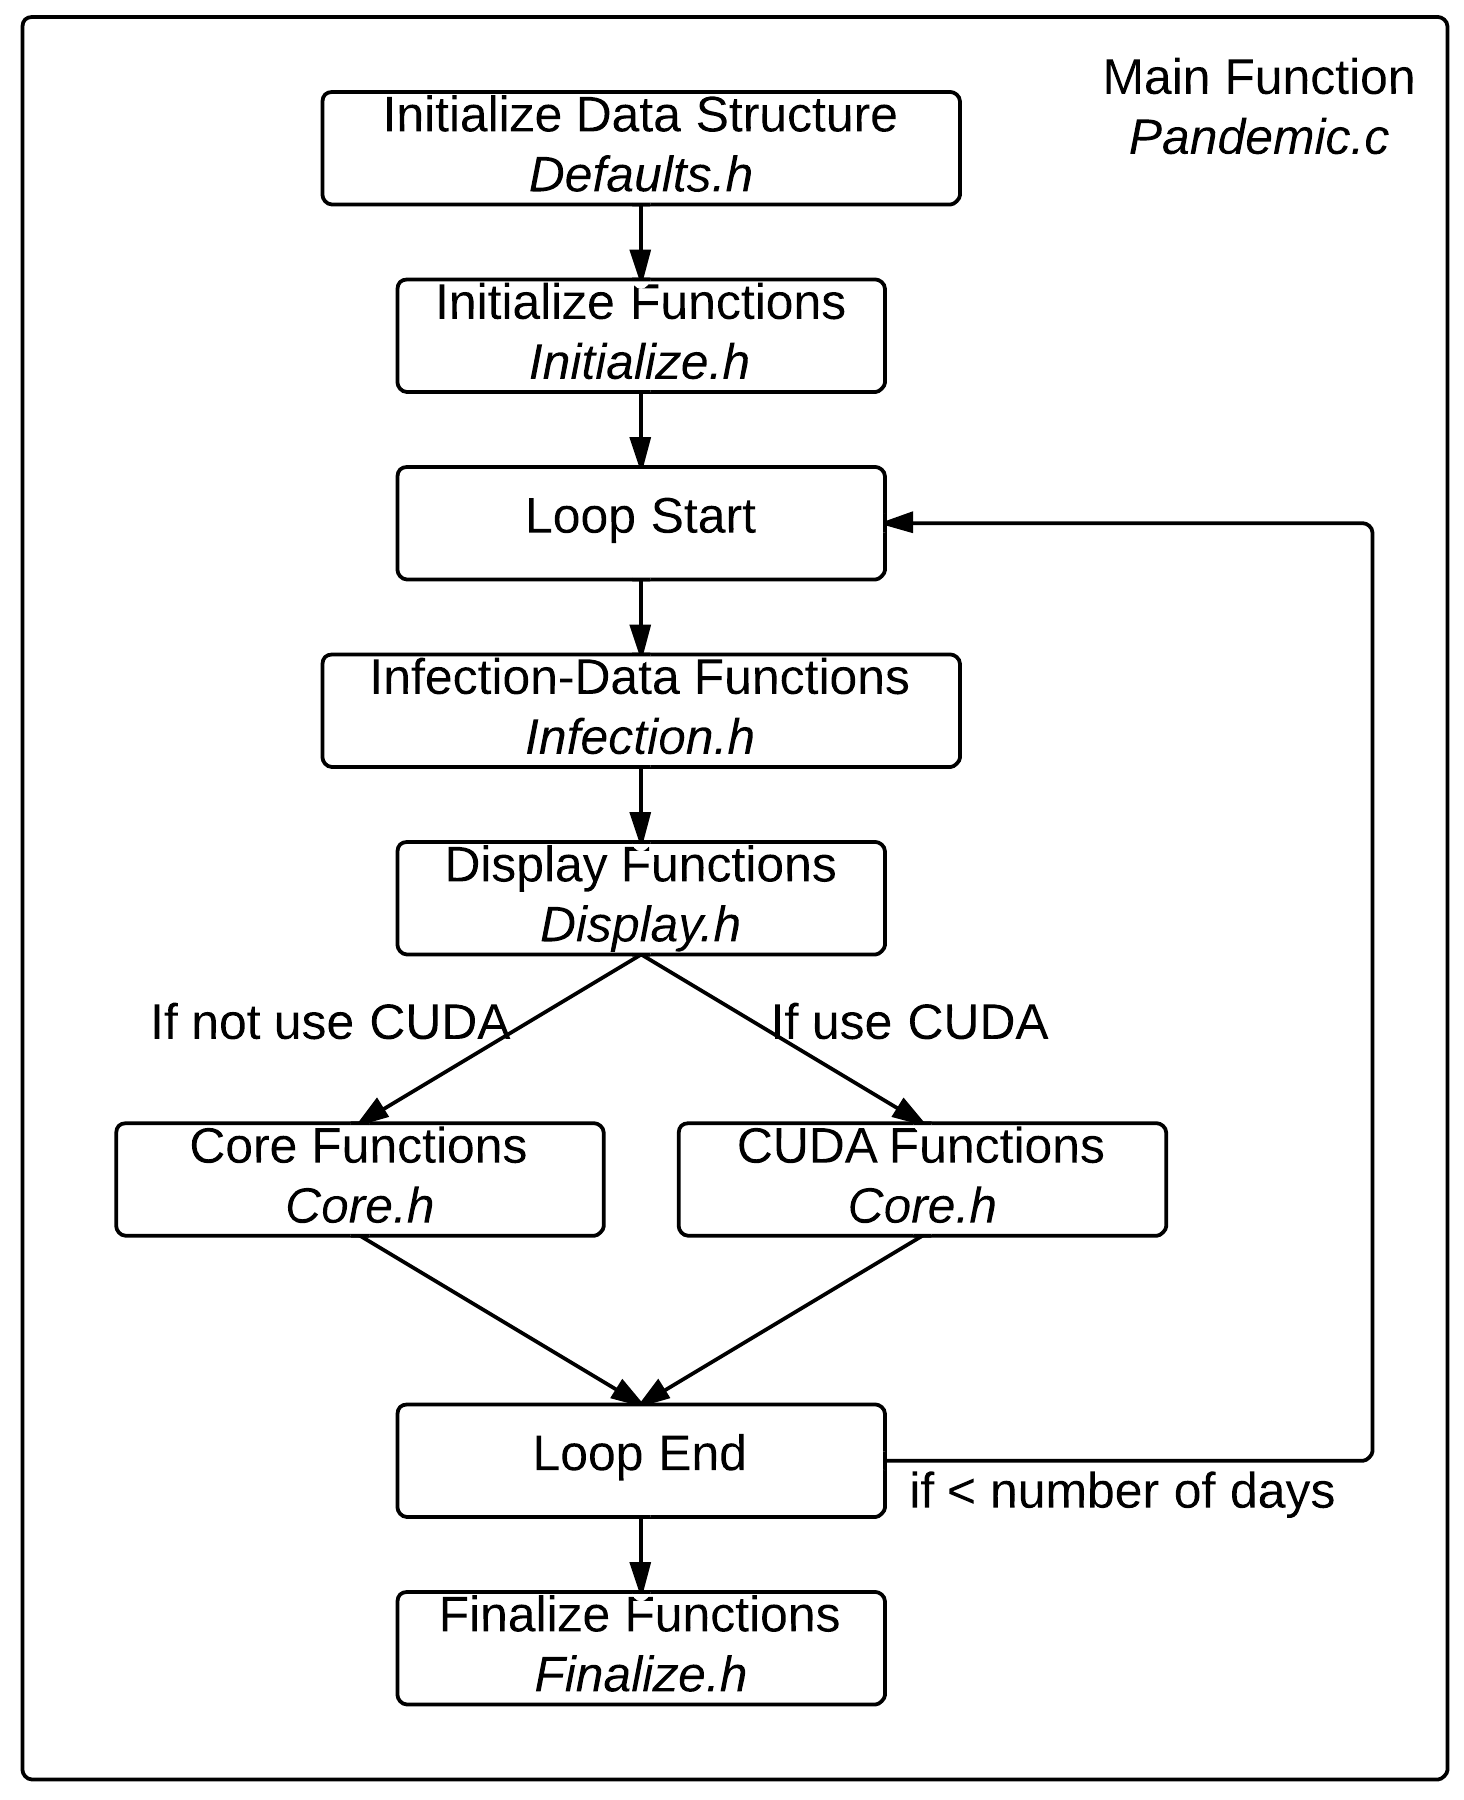
\includegraphics{Structure.png}
\caption{Overall Program Structurer}\end{figure}

The CUDA functions in the \emph{CUDA.cu} file is not included in the file table, even though they are shown in the diagram. The initial serial program does not need these functions or the file. However, we will be using them later in a CUDA version of this code.

The rest of the module will go through each of the code files. We can start with the \emph{Pandemic.c} file.


\section{Pandemic.c}
\label{1-ProgramStructure/programstructure:pandemic-c}
At the very beginning of the file, we need to include all the necessary code files. We first include file files that are needed with our without display.

\begin{Verbatim}[commandchars=\\\{\}]
\PYG{c+cp}{\PYGZsh{}}\PYG{c+cp}{include "Defaults.h"}
\PYG{c+cp}{\PYGZsh{}}\PYG{c+cp}{include "Initialize.h"}
\PYG{c+cp}{\PYGZsh{}}\PYG{c+cp}{include "Infection.h"}
\PYG{c+cp}{\PYGZsh{}}\PYG{c+cp}{include "Core.h"}
\PYG{c+cp}{\PYGZsh{}}\PYG{c+cp}{include "Finalize.h"}
\end{Verbatim}

Then, if we are using display, we include the display code file.

\begin{Verbatim}[commandchars=\\\{\}]
\PYG{c+cp}{\PYGZsh{}}\PYG{c+cp}{if defined(X\PYGZus{}DISPLAY) \textbar{}\textbar{} defined(TEXT\PYGZus{}DISPLAY)}
\PYG{c+cp}{\PYGZsh{}}\PYG{c+cp}{include "Display.h"}
\PYG{c+cp}{\PYGZsh{}}\PYG{c+cp}{endif}
\end{Verbatim}


\subsection{main()}
\label{1-ProgramStructure/programstructure:main}
This function is the backbone of the whole program. It first initialize all the data structures need.

\begin{Verbatim}[commandchars=\\\{\}]
    \PYG{c+cm}{/**** In Defaults.h ****/}
    \PYG{k}{struct} \PYG{n}{global\PYGZus{}t} \PYG{n}{global}\PYG{p}{;}
    \PYG{k}{struct} \PYG{n}{const\PYGZus{}t} \PYG{n}{constant}\PYG{p}{;}
    \PYG{k}{struct} \PYG{n}{stats\PYGZus{}t} \PYG{n}{stats}\PYG{p}{;}
    \PYG{k}{struct} \PYG{n}{display\PYGZus{}t} \PYG{n}{dpy}\PYG{p}{;}
    \PYG{c+cm}{/***********************/}
\end{Verbatim}

Then it will initialize the runtime environment by calling \textbf{init()} function.

\begin{Verbatim}[commandchars=\\\{\}]
    \PYG{c+cm}{/***************** In Initialize.h *****************/}
    \PYG{n}{init}\PYG{p}{(}\PYG{o}{\PYGZam{}}\PYG{n}{global}\PYG{p}{,} \PYG{o}{\PYGZam{}}\PYG{n}{constant}\PYG{p}{,} \PYG{o}{\PYGZam{}}\PYG{n}{stats}\PYG{p}{,} \PYG{o}{\PYGZam{}}\PYG{n}{dpy}\PYG{p}{,} \PYG{o}{\PYGZam{}}\PYG{n}{argc}\PYG{p}{,} \PYG{o}{\PYGZam{}}\PYG{n}{argv}\PYG{p}{)}\PYG{p}{;}
    \PYG{c+cm}{/***************************************************/}
\end{Verbatim}

Then we start the simulation. A for loop wraps around most of the functions, where the each iteration of the loop represents a day passing.

\begin{Verbatim}[commandchars=\\\{\}]
    \PYG{k}{for}\PYG{p}{(}\PYG{n}{global}\PYG{p}{.}\PYG{n}{current\PYGZus{}day} \PYG{o}{=} \PYG{l+m+mi}{0}\PYG{p}{;} \PYG{n}{global}\PYG{p}{.}\PYG{n}{current\PYGZus{}day} \PYG{o}{\PYGZlt{}}\PYG{o}{=} \PYG{n}{constant}\PYG{p}{.}\PYG{n}{total\PYGZus{}number\PYGZus{}of\PYGZus{}days}\PYG{p}{;} 
        \PYG{n}{global}\PYG{p}{.}\PYG{n}{current\PYGZus{}day}\PYG{o}{+}\PYG{o}{+}\PYG{p}{)}
    \PYG{p}{\PYGZob{}}
    \PYG{p}{\PYGZcb{}}
\end{Verbatim}

Inside the for loop, we first find all data related to the infection.

\begin{Verbatim}[commandchars=\\\{\}]
        \PYG{c+cm}{/****** In Infection.h ******/}
        \PYG{n}{find\PYGZus{}infected}\PYG{p}{(}\PYG{o}{\PYGZam{}}\PYG{n}{global}\PYG{p}{)}\PYG{p}{;}
        \PYG{c+cm}{/****************************/}
\end{Verbatim}

Then, if display is enabled, we display the infection status. In other words, we display everyone's location and their states of infection.

\begin{Verbatim}[commandchars=\\\{\}]
        \PYG{c+cm}{/**************** In Display.h *****************/}
        \PYG{c+cp}{\PYGZsh{}}\PYG{c+cp}{if defined(X\PYGZus{}DISPLAY) \textbar{}\textbar{} defined(TEXT\PYGZus{}DISPLAY)}

        \PYG{n}{do\PYGZus{}display}\PYG{p}{(}\PYG{o}{\PYGZam{}}\PYG{n}{global}\PYG{p}{,} \PYG{o}{\PYGZam{}}\PYG{n}{constant}\PYG{p}{,} \PYG{o}{\PYGZam{}}\PYG{n}{dpy}\PYG{p}{)}\PYG{p}{;}

        \PYG{n}{throttle}\PYG{p}{(}\PYG{o}{\PYGZam{}}\PYG{n}{constant}\PYG{p}{)}\PYG{p}{;}

        \PYG{c+cp}{\PYGZsh{}}\PYG{c+cp}{endif}
        \PYG{c+cm}{/***********************************************/}
\end{Verbatim}

After display, we can call four core functions in \emph{Core.h*} code file.

\begin{Verbatim}[commandchars=\\\{\}]
        \PYG{c+cm}{/************** In Core.h *************/}
        \PYG{n}{move}\PYG{p}{(}\PYG{o}{\PYGZam{}}\PYG{n}{global}\PYG{p}{,} \PYG{o}{\PYGZam{}}\PYG{n}{constant}\PYG{p}{)}\PYG{p}{;}       

        \PYG{n}{susceptible}\PYG{p}{(}\PYG{o}{\PYGZam{}}\PYG{n}{global}\PYG{p}{,} \PYG{o}{\PYGZam{}}\PYG{n}{constant}\PYG{p}{,} \PYG{o}{\PYGZam{}}\PYG{n}{stats}\PYG{p}{)}\PYG{p}{;}

        \PYG{n}{infected}\PYG{p}{(}\PYG{o}{\PYGZam{}}\PYG{n}{global}\PYG{p}{,} \PYG{o}{\PYGZam{}}\PYG{n}{constant}\PYG{p}{,} \PYG{o}{\PYGZam{}}\PYG{n}{stats}\PYG{p}{)}\PYG{p}{;}

        \PYG{n}{update\PYGZus{}days\PYGZus{}infected}\PYG{p}{(}\PYG{o}{\PYGZam{}}\PYG{n}{global}\PYG{p}{,} \PYG{o}{\PYGZam{}}\PYG{n}{constant}\PYG{p}{)}\PYG{p}{;}
        \PYG{c+cm}{/**************************************/}
\end{Verbatim}

This is the end of the loop.

Finally, after the loop, we can display the results and finalize the runtime environment.

\begin{Verbatim}[commandchars=\\\{\}]
    \PYG{c+cm}{/******** In Finialize.h ********/}
    \PYG{n}{show\PYGZus{}results}\PYG{p}{(}\PYG{o}{\PYGZam{}}\PYG{n}{global}\PYG{p}{,} \PYG{o}{\PYGZam{}}\PYG{n}{stats}\PYG{p}{)}\PYG{p}{;}

    \PYG{n}{cleanup}\PYG{p}{(}\PYG{o}{\PYGZam{}}\PYG{n}{global}\PYG{p}{,} \PYG{o}{\PYGZam{}}\PYG{n}{constant}\PYG{p}{,} \PYG{o}{\PYGZam{}}\PYG{n}{dpy}\PYG{p}{)}\PYG{p}{;}
    \PYG{c+cm}{/********************************/}
\end{Verbatim}


\chapter{Data Structures}
\label{2-DataStructure/datastructure:data-structures}\label{2-DataStructure/datastructure::doc}
Here is the list of variables and arrays used by the program. Note the
naming scheme; variables whose names begin with “my” are private to the
threads that use them. Variables whose names begin with “our” are
private to the processes that use them, but public to the threads within
that process. Variables are thus named from a thread’s perspective; “my”
variables are ones that I use, “our” variables are ones that I and the
other threads in my process use.


\section{display\_t struct}
\label{2-DataStructure/datastructure:display-t-struct}
\begin{Verbatim}[commandchars=\\\{\}]
\PYG{c+c1}{// Data being used for the X display}
\PYG{k}{struct} \PYG{n}{display\PYGZus{}t} \PYG{p}{\PYGZob{}}

	\PYG{c+cp}{\PYGZsh{}}\PYG{c+cp}{ifdef TEXT\PYGZus{}DISPLAY}
    \PYG{c+c1}{// Array of character arrays for text display }
	\PYG{k+kt}{char} \PYG{o}{*}\PYG{o}{*}\PYG{n}{environment}\PYG{p}{;}
	\PYG{c+cp}{\PYGZsh{}}\PYG{c+cp}{endif}

	\PYG{c+cp}{\PYGZsh{}}\PYG{c+cp}{ifdef X\PYGZus{}DISPLAY}
	\PYG{c+c1}{// Declare X-related variables }
	\PYG{n}{Display}   		\PYG{o}{*}\PYG{n}{display}\PYG{p}{;}
	\PYG{n}{Window}    		\PYG{n}{window}\PYG{p}{;}
	\PYG{k+kt}{int} 			\PYG{n}{screen}\PYG{p}{;}
	\PYG{n}{Atom} 			\PYG{n}{delete\PYGZus{}window}\PYG{p}{;}
	\PYG{n}{GC}        		\PYG{n}{gc}\PYG{p}{;}
	\PYG{n}{XColor} 			\PYG{n}{infected\PYGZus{}color}\PYG{p}{;}
	\PYG{n}{XColor} 			\PYG{n}{immune\PYGZus{}color}\PYG{p}{;}
	\PYG{n}{XColor} 			\PYG{n}{susceptible\PYGZus{}color}\PYG{p}{;}
	\PYG{n}{XColor} 			\PYG{n}{dead\PYGZus{}color}\PYG{p}{;}
	\PYG{n}{Colormap} 		\PYG{n}{colormap}\PYG{p}{;}
	\PYG{k+kt}{char} 			\PYG{o}{*}\PYG{n}{red}\PYG{p}{;}
	\PYG{k+kt}{char} 			\PYG{o}{*}\PYG{n}{green}\PYG{p}{;}
	\PYG{k+kt}{char} 			\PYG{o}{*}\PYG{n}{black}\PYG{p}{;}
	\PYG{k+kt}{char} 			\PYG{o}{*}\PYG{n}{white}\PYG{p}{;}
	\PYG{c+cp}{\PYGZsh{}}\PYG{c+cp}{endif}
\PYG{p}{\PYGZcb{}}\PYG{p}{;}
\end{Verbatim}

\textbf{environment}

2D array, holds an ASCII representation of the environment (see “state” under “Person” in the “Model” section). This variable is used only when we are using Text Display.

\textbf{display}

Display, display pointer for the connection to the X server

\textbf{window}

Window, variable to hold the window id.

\textbf{screen}

Screen, variable to hold default screen

\textbf{delete\_window}

\textbf{gc}

\textbf{infected\_color}

\textbf{immune\_color}

\textbf{susceptible\_color}

\textbf{dead\_color}

\textbf{red}

array of char, holds value \#FF0000, which is the hex code for color red.

\textbf{green}

array of char, holds value \#00FF00, which is the hex code for color green.

\textbf{black}

array of char, holds value \#000000, which is the hex code for color black.

\textbf{white}

array of char, holds value \#FFFFFF, which is the hex code for color white.

\textbf{colormap}


\section{global\_t struct}
\label{2-DataStructure/datastructure:global-t-struct}
\begin{Verbatim}[commandchars=\\\{\}]
\PYG{c+c1}{// All the data needed globally. Holds EVERYONE's location, }
\PYG{c+c1}{// states and other necessary counters.}
\PYG{k}{struct} \PYG{n}{global\PYGZus{}t} 
\PYG{p}{\PYGZob{}}
	\PYG{c+c1}{// current day}
	\PYG{k+kt}{int} \PYG{n}{current\PYGZus{}day}\PYG{p}{;}
	\PYG{c+c1}{// people counters}
	\PYG{k+kt}{int} \PYG{n}{number\PYGZus{}of\PYGZus{}people}\PYG{p}{;}
	\PYG{k+kt}{int} \PYG{n}{num\PYGZus{}initially\PYGZus{}infected}\PYG{p}{;}
	\PYG{c+c1}{// states counters}
	\PYG{k+kt}{int} \PYG{n}{num\PYGZus{}infected}\PYG{p}{;}
	\PYG{k+kt}{int} \PYG{n}{num\PYGZus{}susceptible}\PYG{p}{;}
	\PYG{k+kt}{int} \PYG{n}{num\PYGZus{}immune}\PYG{p}{;}
	\PYG{k+kt}{int} \PYG{n}{num\PYGZus{}dead}\PYG{p}{;}  
	\PYG{c+c1}{// locations}
	\PYG{k+kt}{int} \PYG{o}{*}\PYG{n}{x\PYGZus{}locations}\PYG{p}{;}
	\PYG{k+kt}{int} \PYG{o}{*}\PYG{n}{y\PYGZus{}locations}\PYG{p}{;}
	\PYG{c+c1}{// infected people's locations}
	\PYG{k+kt}{int} \PYG{o}{*}\PYG{n}{infected\PYGZus{}x\PYGZus{}locations}\PYG{p}{;}
	\PYG{k+kt}{int} \PYG{o}{*}\PYG{n}{infected\PYGZus{}y\PYGZus{}locations}\PYG{p}{;}
	\PYG{c+c1}{// state}
	\PYG{k+kt}{char} \PYG{o}{*}\PYG{n}{states}\PYG{p}{;}
	\PYG{c+c1}{// infected time}
	\PYG{k+kt}{int} \PYG{o}{*}\PYG{n}{num\PYGZus{}days\PYGZus{}infected}\PYG{p}{;}
\PYG{p}{\PYGZcb{}}\PYG{p}{;}
\end{Verbatim}

\textbf{current\_day}

a loop iterator representing the ID of the current day being simulated by the current process.

\textbf{number\_of\_people}

the total number of all people in the simulation. The value of this variable can be specified on the command line with the –n option.

\textbf{num\_initially\_infected}

the total number of people who are initially infected. The value of this variable can be specified on the command line with the –i option. This is a subset of the total number of people, so the value of this variable must be smaller or equal to the value for \textbf{number\_of\_people}.

\textbf{num\_infected}

acount of the number of infected people. This value changes throughout the course of the simulation.

\textbf{num\_susceptible}

acount of the number of susceptible people. This value changes throughout the course of the simulation.

\textbf{our\_num\_immune}

acount of the number of immune people. This value changes throughout the course of the simulation.

\textbf{our\_num\_dead}

acount of the number of dead people. This value changes throughout the course of the simulation.

\textbf{x\_locations}

array, holds the x locations of all of the people; used if the environment needs to be displayed.

\textbf{y\_locations}

array, holds the y locations of all of the people; used if the environment needs to be displayed.

\textbf{infected\_x\_locations}

array, used in \textbf{susceptible()} to keep track of the x locations of the infected people.

\textbf{infected\_y\_locations}

array, used in \textbf{susceptible()} to keep track of the y locations of the infected people.

\textbf{states}

array, holds the states of all of the people; used if the environment needs to be displayed.

\textbf{num\_days\_infected}

array, used to keep track of the number of days each person has been infected.


\section{const\_t struct}
\label{2-DataStructure/datastructure:const-t-struct}
\begin{Verbatim}[commandchars=\\\{\}]
\PYG{k}{struct} \PYG{n}{const\PYGZus{}t} 
\PYG{p}{\PYGZob{}}
    \PYG{c+c1}{// environment}
    \PYG{k+kt}{int} \PYG{n}{environment\PYGZus{}width}\PYG{p}{;}
    \PYG{k+kt}{int} \PYG{n}{environment\PYGZus{}height}\PYG{p}{;}
    \PYG{c+c1}{// disease}
    \PYG{k+kt}{int} \PYG{n}{infection\PYGZus{}radius}\PYG{p}{;}
    \PYG{k+kt}{int} \PYG{n}{duration\PYGZus{}of\PYGZus{}disease}\PYG{p}{;}
    \PYG{k+kt}{int} \PYG{n}{contagiousness\PYGZus{}factor}\PYG{p}{;}
    \PYG{k+kt}{int} \PYG{n}{deadliness\PYGZus{}factor}\PYG{p}{;}
    \PYG{c+c1}{// time}
    \PYG{k+kt}{int} \PYG{n}{total\PYGZus{}number\PYGZus{}of\PYGZus{}days}\PYG{p}{;}
    \PYG{k+kt}{int} \PYG{n}{microseconds\PYGZus{}per\PYGZus{}day}\PYG{p}{;}
\PYG{p}{\PYGZcb{}}\PYG{p}{;}
\end{Verbatim}

\textbf{environment\_width}

environment\_width – indicates how wide the environment is; used to draw
the environment and to make sure people stay within the bounds of the
environment.

\textbf{environment\_height}

environment\_height – indicates how high the environment is; used to
draw the environment and to make sure people stay within the bounds of
the environment.

\textbf{infection\_radius}

see the introduction chapter. The value of this
variable can be specified on the command line with the –d option.

\textbf{duration\_of\_disease}

see the introduction chapter. The value of this
variable can be specified on the command line with the –T option.

\textbf{contagiousness\_factor}

see the introduction chapter. The value of this
variable can be specified on the command line with the –c option.

\textbf{deadliness\_factor}

see the introduction chapter. The value of this
variable can be specified on the command line with the –D option.

\textbf{total\_number\_of\_days}

the total number of days over which to run the simulation.

\textbf{microseconds\_per\_day}

used to tell how many microseconds to freeze in between frames of animation. The value of this variable can be specified on the command line with the –m option.


\section{stats\_t struct}
\label{2-DataStructure/datastructure:stats-t-struct}
\begin{Verbatim}[commandchars=\\\{\}]
\PYG{c+c1}{// Data being used for SHOW\PYGZus{}RESULTS}
\PYG{k}{struct} \PYG{n}{stats\PYGZus{}t} 
\PYG{p}{\PYGZob{}}
    \PYG{k+kt}{double} \PYG{n}{num\PYGZus{}infections}\PYG{p}{;}
    \PYG{k+kt}{double} \PYG{n}{num\PYGZus{}infection\PYGZus{}attempts}\PYG{p}{;}
    \PYG{k+kt}{double} \PYG{n}{num\PYGZus{}deaths}\PYG{p}{;}
    \PYG{k+kt}{double} \PYG{n}{num\PYGZus{}recovery\PYGZus{}attempts}\PYG{p}{;} 
\PYG{p}{\PYGZcb{}}\PYG{p}{;}
\end{Verbatim}

\textbf{our\_num\_infections}

used to count the number of actual infections
that take place (in which an infected person transmits the disease to a
susceptible person). Only used if the showing of results is enabled
(i.e., if the program is to print out final results from the
simulation). Used to determine the actual contagiousness of the disease,
which can be compared to the contagiousness factor by the user.

\textbf{our\_num\_infection\_attempts}

used to count the number of times a
susceptible person is within an infection radius of an infected person,
even if the infection fails. Only used if the showing of results is
enabled (i.e., if the program is to print out final results from the
simulation). Used to determine the actual contagiousness of the disease,
which can be compared to the contagiousness factor by the user.

\textbf{our\_num\_deaths}

used to count the number of times a person dies. Only
used if the showing of results is enabled (i.e., if the program is to
print out final results from the simulation). Used to determine the
actual deadliness of the disease, which can be compared to the
deadliness factor by the user.

\textbf{our\_num\_recovery\_attempts}

used to count the number of times an
infected person is able to become immune. Only used if the showing of
results is enabled (i.e., if the program is to print out final results
from the simulation). Used to determine the actual deadliness of the
disease, which can be compared to the deadliness factor by the user.


\chapter{Initialize Functions}
\label{3-Initialize/initialize:initialize-functions}\label{3-Initialize/initialize::doc}

\section{init}
\label{3-Initialize/initialize:init}
This function will first initialize variables in the constant structure with default values. It will also initialize \textbf{number\_of\_people} variable and \textbf{num\_initially\_infected} variable. After this, it will set all the counters in side stats structure to zero, as well as state counters inside global struct.

Then, \textbf{Init()} function will call the following 5 functions to finish the initialization process.


\section{parse\_args}
\label{3-Initialize/initialize:parse-args}\begin{figure}[htbp]
\centering

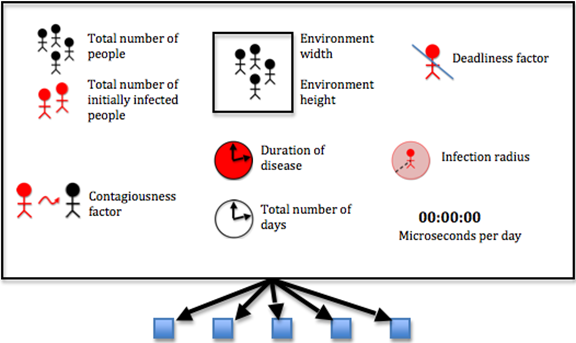
\includegraphics{img-6.png}
\end{figure}

These parameters are specified via command line arguments when the
program is run. Otherwise, default values are used. The code uses \textbf{getopt}
function to do this. Type \textbf{man 3 getopt} in a shell if you are interested
how it works.


\section{init\_check}
\label{3-Initialize/initialize:init-check}
This function makes sure that the \textbf{total number of initially infected people} is less than the \textbf{total number of people}
\begin{figure}[htbp]
\centering

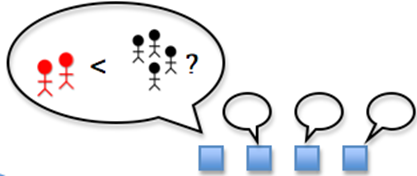
\includegraphics{img-7.png}
\end{figure}

The simulation can’t run if there are more initially infected people
than there are people. If there are, the code uses the fprintf function
to print an error message to standard error, and it exits the program
with exit code -1.


\section{allocate\_array}
\label{3-Initialize/initialize:allocate-array}
At this point we are ready to allocate our arrays, which must be performed before we can start filling the arrays. Allocating an array means reserving enough space in memory for it; if we don’t reserve the space the program will assume that it is a zero-length array. The allocation must happen in the “heap” memory, meaning we must allocate it dynamically (i.e. as the program is running). To allocate memory on the heap, we use the \textbf{malloc} function, which takes the amount of space that is requested and returns a pointer to the newly allocated memory, which we can then use as an array. Let’s see an example with the \textbf{x\_locations} array:

\begin{Verbatim}[commandchars=\\\{\}]
    \PYG{n}{global}\PYG{o}{-}\PYG{o}{\PYGZgt{}}\PYG{n}{x\PYGZus{}locations} \PYG{o}{=} \PYG{p}{(}\PYG{k+kt}{int}\PYG{o}{*}\PYG{p}{)}\PYG{n}{malloc}\PYG{p}{(}\PYG{n}{number\PYGZus{}of\PYGZus{}people} \PYG{o}{*} \PYG{k}{sizeof}\PYG{p}{(}\PYG{k+kt}{int}\PYG{p}{)}\PYG{p}{)}\PYG{p}{;}
\end{Verbatim}

Here we see that malloc has taken an argument, \textbf{number\_of\_people
* sizeof(int)}. This is how we specify that we want to fill the array
with a certain number of integers, namely the amount stored in the
\textbf{number\_of\_people} variable. We also need to specify how big
these integers are, for which we use the \textbf{sizeof(int)} function. We then
take the return from \textbf{malloc} and tell the program to “cast” it (i.e. use
it) as a pointer to integers, for which we use \textbf{(int*)}. This is then
assigned to \textbf{x\_locations}, and we can now use \textbf{x\_locations} as an array.

For the 2D array \textbf{environment}, we must allocate not only the array itself
but also each of the arrays that it contains (since a 2D array is an
array whose elements are arrays). The array has horizontal strips of
length \textbf{environment\_width} and vertical strips of length
\textbf{environment\_height}. We perform the allocation by allocating enough
space for the entire array first using

\begin{Verbatim}[commandchars=\\\{\}]
    \PYG{n}{dpy}\PYG{o}{-}\PYG{o}{\PYGZgt{}}\PYG{n}{environment} \PYG{o}{=} \PYG{p}{(}\PYG{k+kt}{char}\PYG{o}{*}\PYG{o}{*}\PYG{p}{)}\PYG{n}{malloc}\PYG{p}{(}\PYG{n}{constant}\PYG{o}{-}\PYG{o}{\PYGZgt{}}\PYG{n}{environment\PYGZus{}width} \PYG{o}{*} 
        \PYG{n}{constant}\PYG{o}{-}\PYG{o}{\PYGZgt{}}\PYG{n}{environment\PYGZus{}height} \PYG{o}{*} \PYG{k}{sizeof}\PYG{p}{(}\PYG{k+kt}{char}\PYG{o}{*}\PYG{p}{)}\PYG{p}{)}\PYG{p}{;}
\end{Verbatim}

That is, we are allocating enough \textbf{char*}’s for
\textbf{environment\_width} times \textbf{environment\_height}, casting this as a \textbf{char**}
and assigning it to \textbf{environment}. Then we allocate each array within
\textbf{environment}, like so:

\begin{Verbatim}[commandchars=\\\{\}]
    \PYG{n}{dpy}\PYG{o}{-}\PYG{o}{\PYGZgt{}}\PYG{n}{environment} \PYG{o}{=} \PYG{p}{(}\PYG{k+kt}{char}\PYG{o}{*}\PYG{o}{*}\PYG{p}{)}\PYG{n}{malloc}\PYG{p}{(}\PYG{n}{constant}\PYG{o}{-}\PYG{o}{\PYGZgt{}}\PYG{n}{environment\PYGZus{}width} \PYG{o}{*} 
        \PYG{n}{constant}\PYG{o}{-}\PYG{o}{\PYGZgt{}}\PYG{n}{environment\PYGZus{}height} \PYG{o}{*} \PYG{k}{sizeof}\PYG{p}{(}\PYG{k+kt}{char}\PYG{o}{*}\PYG{p}{)}\PYG{p}{)}\PYG{p}{;}
    \PYG{k+kt}{int} \PYG{n}{current\PYGZus{}location\PYGZus{}x}\PYG{p}{;}
    \PYG{k}{for}\PYG{p}{(}\PYG{n}{current\PYGZus{}location\PYGZus{}x} \PYG{o}{=} \PYG{l+m+mi}{0}\PYG{p}{;} 
        \PYG{n}{current\PYGZus{}location\PYGZus{}x} \PYG{o}{\PYGZlt{}}\PYG{o}{=} \PYG{n}{constant}\PYG{o}{-}\PYG{o}{\PYGZgt{}}\PYG{n}{environment\PYGZus{}width} \PYG{o}{-} \PYG{l+m+mi}{1}\PYG{p}{;}
            \PYG{n}{current\PYGZus{}location\PYGZus{}x}\PYG{o}{+}\PYG{o}{+}\PYG{p}{)}
    \PYG{p}{\PYGZob{}}
        \PYG{n}{dpy}\PYG{o}{-}\PYG{o}{\PYGZgt{}}\PYG{n}{environment}\PYG{p}{[}\PYG{n}{current\PYGZus{}location\PYGZus{}x}\PYG{p}{]} \PYG{o}{=} \PYG{p}{(}\PYG{k+kt}{char}\PYG{o}{*}\PYG{p}{)}\PYG{n}{malloc}\PYG{p}{(}
            \PYG{n}{constant}\PYG{o}{-}\PYG{o}{\PYGZgt{}}\PYG{n}{environment\PYGZus{}height} \PYG{o}{*} \PYG{k}{sizeof}\PYG{p}{(}\PYG{k+kt}{char}\PYG{p}{)}\PYG{p}{)}\PYG{p}{;}
    \PYG{p}{\PYGZcb{}}
\end{Verbatim}

The number of arrays we need is stored in \textbf{environment\_width}, so we loop
from \textbf{0} to \textbf{environment\_width – 1} and allocate enough space in each
element of environment for \textbf{environment\_height} chars, each one of which
has size \textbf{sizeof(char)}.

This can be a convoluted process but is necessary for allocating arrays
dynamically, which allows us to specify options on the command line (so
we don’t have to edit the source code and re-compile each time we want
to run a simulation with different parameters).


\section{init\_array}
\label{3-Initialize/initialize:init-array}
First, the function set the states of the initially infected people and set the count of its infected people
\begin{figure}[htbp]
\centering

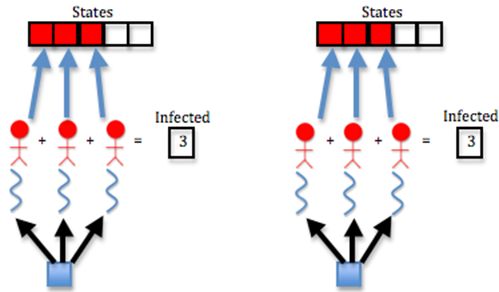
\includegraphics{img-12.png}
\end{figure}

Threads set the states of infected people using the \textbf{states} array.
They fill the first \textbf{num\_initially\_infected} cells of the array
with the \textbf{INFECTED} constant; i.e. they fill in the \textbf{0} through
\textbf{num\_initially\_infected – 1} positions of the array with \textbf{INFECTED}
as below:

\begin{Verbatim}[commandchars=\\\{\}]
    \PYG{c+c1}{// Each process spawns threads to set the states of the initially }
    \PYG{c+c1}{// infected people and set the count of its infected people}
    \PYG{k}{for}\PYG{p}{(}\PYG{n}{current\PYGZus{}person\PYGZus{}id} \PYG{o}{=} \PYG{l+m+mi}{0}\PYG{p}{;} \PYG{n}{current\PYGZus{}person\PYGZus{}id} 
        \PYG{o}{\PYGZlt{}}\PYG{o}{=} \PYG{n}{num\PYGZus{}initially\PYGZus{}infected} \PYG{o}{-} \PYG{l+m+mi}{1}\PYG{p}{;} \PYG{n}{current\PYGZus{}person\PYGZus{}id}\PYG{o}{+}\PYG{o}{+}\PYG{p}{)}
    \PYG{p}{\PYGZob{}}
        \PYG{n}{global}\PYG{o}{-}\PYG{o}{\PYGZgt{}}\PYG{n}{states}\PYG{p}{[}\PYG{n}{current\PYGZus{}person\PYGZus{}id}\PYG{p}{]} \PYG{o}{=} \PYG{n}{INFECTED}\PYG{p}{;}
        \PYG{n}{global}\PYG{o}{-}\PYG{o}{\PYGZgt{}}\PYG{n}{num\PYGZus{}infected}\PYG{o}{+}\PYG{o}{+}\PYG{p}{;}
    \PYG{p}{\PYGZcb{}}
\end{Verbatim}

Note we also add 1 to the \textbf{num\_infected variable} using the plus-plus operator (++) at each iteration of the loop. This is how we count the number of infected people.

Next, the function set the states of the rest of its people and set the count of its susceptible people
\begin{figure}[htbp]
\centering

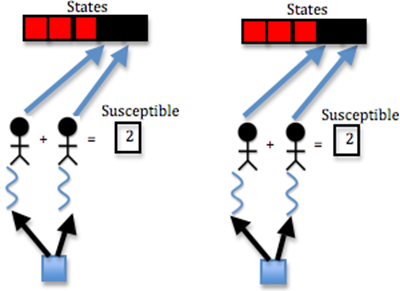
\includegraphics{img-13.png}
\end{figure}

This is similar to last step, but we want to fill the rest of the array
(from \textbf{num\_initially\_infected} to \textbf{number\_of\_people - 1}) with
the \textbf{SUSCEPTIBLE} constant, and we want to add \textbf{1} to the
\textbf{num\_susceptible} variable at each iteration of the loop:

\begin{Verbatim}[commandchars=\\\{\}]
    \PYG{c+c1}{// Each process spawns threads to set the states of the rest of}
    \PYG{c+c1}{// its people and set the count of its susceptible people}
    \PYG{k}{for}\PYG{p}{(}\PYG{n}{current\PYGZus{}person\PYGZus{}id} \PYG{o}{=} \PYG{n}{num\PYGZus{}initially\PYGZus{}infected}\PYG{p}{;} 
        \PYG{n}{current\PYGZus{}person\PYGZus{}id} \PYG{o}{\PYGZlt{}}\PYG{o}{=} \PYG{n}{number\PYGZus{}of\PYGZus{}people} \PYG{o}{-} \PYG{l+m+mi}{1}\PYG{p}{;} 
        \PYG{n}{current\PYGZus{}person\PYGZus{}id}\PYG{o}{+}\PYG{o}{+}\PYG{p}{)}
    \PYG{p}{\PYGZob{}}
        \PYG{n}{global}\PYG{o}{-}\PYG{o}{\PYGZgt{}}\PYG{n}{states}\PYG{p}{[}\PYG{n}{current\PYGZus{}person\PYGZus{}id}\PYG{p}{]} \PYG{o}{=} \PYG{n}{SUSCEPTIBLE}\PYG{p}{;}
        \PYG{n}{global}\PYG{o}{-}\PYG{o}{\PYGZgt{}}\PYG{n}{num\PYGZus{}susceptible}\PYG{o}{+}\PYG{o}{+}\PYG{p}{;}
    \PYG{p}{\PYGZcb{}}
\end{Verbatim}

The \textbf{states} array is now full; the first \textbf{num\_initially\_infected} cells have the \textbf{INFECTED} constant, and the rest have the \textbf{SUSCEPTIBLE} constant.

Then, the function sets random x and y locations for each people
\begin{figure}[htbp]
\centering

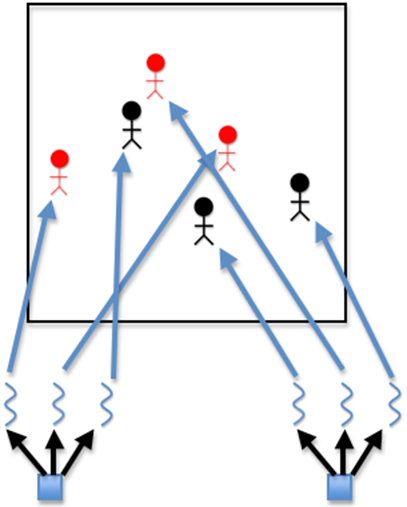
\includegraphics{img-14.png}
\end{figure}

Locations of people are stored in the \textbf{x\_locations} and \textbf{y\_locations} arrays. To fill these arrays with random values, we use a for loop and the random function:

\begin{Verbatim}[commandchars=\\\{\}]
    \PYG{c+c1}{// Each process spawns threads to set random x and y locations for }
    \PYG{c+c1}{// each of its people}
    \PYG{k}{for}\PYG{p}{(}\PYG{n}{current\PYGZus{}person\PYGZus{}id} \PYG{o}{=} \PYG{l+m+mi}{0}\PYG{p}{;}
        \PYG{n}{current\PYGZus{}person\PYGZus{}id} \PYG{o}{\PYGZlt{}}\PYG{o}{=} \PYG{n}{number\PYGZus{}of\PYGZus{}people} \PYG{o}{-} \PYG{l+m+mi}{1}\PYG{p}{;} 
        \PYG{n}{current\PYGZus{}person\PYGZus{}id}\PYG{o}{+}\PYG{o}{+}\PYG{p}{)}
    \PYG{p}{\PYGZob{}}
        \PYG{n}{global}\PYG{o}{-}\PYG{o}{\PYGZgt{}}\PYG{n}{x\PYGZus{}locations}\PYG{p}{[}\PYG{n}{current\PYGZus{}person\PYGZus{}id}\PYG{p}{]} \PYG{o}{=} \PYG{n}{random}\PYG{p}{(}\PYG{p}{)} \PYG{o}{\PYGZpc{}} \PYG{n}{constant}\PYG{o}{-}\PYG{o}{\PYGZgt{}}\PYG{n}{environment\PYGZus{}width}\PYG{p}{;}
        \PYG{n}{global}\PYG{o}{-}\PYG{o}{\PYGZgt{}}\PYG{n}{y\PYGZus{}locations}\PYG{p}{[}\PYG{n}{current\PYGZus{}person\PYGZus{}id}\PYG{p}{]} \PYG{o}{=} \PYG{n}{random}\PYG{p}{(}\PYG{p}{)} \PYG{o}{\PYGZpc{}} \PYG{n}{constant}\PYG{o}{-}\PYG{o}{\PYGZgt{}}\PYG{n}{environment\PYGZus{}height}\PYG{p}{;}
    \PYG{p}{\PYGZcb{}}
\end{Verbatim}

By calling random with the \textbf{modulus (\%)} operator, we can restrict the
size of the random number it generates. Since we cannot have x locations
larger than the width of the environment, we call \textbf{random() \%
environment\_width}; to make sure the \textbf{x location} of each person is less
than \textbf{environment\_width}. Similarly for the \textbf{y location} and
\textbf{environment\_height}.

We are filling the x and y location arrays for all of the people for
which the process is responsible, so we loop from \textbf{0} to \textbf{number\_of\_people – 1}.

Finally, the function initializes the number of days infected of each of its people to 0
\begin{figure}[htbp]
\centering

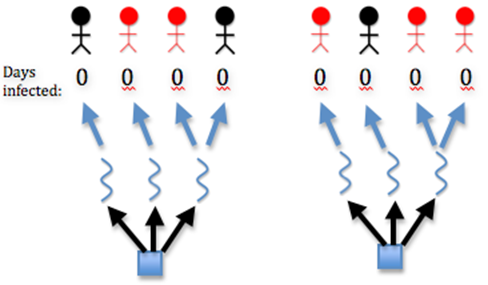
\includegraphics{img-15.png}
\end{figure}

The number of days each person is infected is stored in the \textbf{num\_days\_infected} array, so we loop over all of the people and
fill this array with 0, since the simulation starts at day 0, at which
point no days have yet elapsed:

\begin{Verbatim}[commandchars=\\\{\}]
    \PYG{c+c1}{// Each process spawns threads to initialize the number of days }
    \PYG{c+c1}{// infected of each of its people to 0}
    \PYG{k}{for}\PYG{p}{(}\PYG{n}{current\PYGZus{}person\PYGZus{}id} \PYG{o}{=} \PYG{l+m+mi}{0}\PYG{p}{;}
        \PYG{n}{current\PYGZus{}person\PYGZus{}id} \PYG{o}{\PYGZlt{}}\PYG{o}{=} \PYG{n}{number\PYGZus{}of\PYGZus{}people} \PYG{o}{-} \PYG{l+m+mi}{1}\PYG{p}{;}
        \PYG{n}{current\PYGZus{}person\PYGZus{}id}\PYG{o}{+}\PYG{o}{+}\PYG{p}{)}
    \PYG{p}{\PYGZob{}}
        \PYG{n}{global}\PYG{o}{-}\PYG{o}{\PYGZgt{}}\PYG{n}{num\PYGZus{}days\PYGZus{}infected}\PYG{p}{[}\PYG{n}{current\PYGZus{}person\PYGZus{}id}\PYG{p}{]} \PYG{o}{=} \PYG{l+m+mi}{0}\PYG{p}{;}
    \PYG{p}{\PYGZcb{}}
\end{Verbatim}


\chapter{Infection Functions}
\label{4-Infection/infection:infection-functions}\label{4-Infection/infection::doc}

\section{find\_infected}
\label{4-Infection/infection:find-infected}
This function determines the \textbf{x\_location} and \textbf{y\_location} of all the infected people.
\begin{figure}[htbp]
\centering

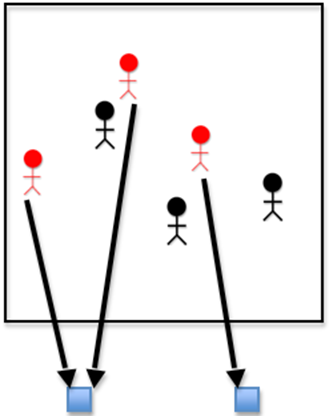
\includegraphics{img-16.png}
\end{figure}

We have already set the states of the infected people and the positions
of all the people, but we need to specifically set the positions of the
infected people and store them in the \textbf{infected\_x\_locations} and
\textbf{infected\_y\_locations} arrays. We do this by marching through the
\textbf{states} array and checking whether the state at each cell is
\textbf{INFECTED}. If it is, we add the locations of the current infected person
from the \textbf{x\_locations} and \textbf{y\_locations} arrays to the
\textbf{infected\_x\_locations} and \textbf{infected\_y\_locations} arrays. We
determine the ID of the current infected person using the
\textbf{current\_infected\_person} variable:

\begin{Verbatim}[commandchars=\\\{\}]
    \PYG{k+kt}{int} \PYG{n}{current\PYGZus{}infected\PYGZus{}person} \PYG{o}{=} \PYG{l+m+mi}{0}\PYG{p}{;}
    \PYG{k}{for}\PYG{p}{(}\PYG{n}{current\PYGZus{}person\PYGZus{}id} \PYG{o}{=} \PYG{l+m+mi}{0}\PYG{p}{;} \PYG{n}{current\PYGZus{}person\PYGZus{}id} \PYG{o}{\PYGZlt{}}\PYG{o}{=} \PYG{n}{global}\PYG{o}{-}\PYG{o}{\PYGZgt{}}\PYG{n}{number\PYGZus{}of\PYGZus{}people} \PYG{o}{-} \PYG{l+m+mi}{1}\PYG{p}{;} 
        \PYG{n}{current\PYGZus{}person\PYGZus{}id}\PYG{o}{+}\PYG{o}{+}\PYG{p}{)}
    \PYG{p}{\PYGZob{}}
        \PYG{k}{if}\PYG{p}{(}\PYG{n}{global}\PYG{o}{-}\PYG{o}{\PYGZgt{}}\PYG{n}{states}\PYG{p}{[}\PYG{n}{current\PYGZus{}person\PYGZus{}id}\PYG{p}{]} \PYG{o}{=}\PYG{o}{=} \PYG{n}{INFECTED}\PYG{p}{)}
        \PYG{p}{\PYGZob{}}
            \PYG{n}{global}\PYG{o}{-}\PYG{o}{\PYGZgt{}}\PYG{n}{infected\PYGZus{}x\PYGZus{}locations}\PYG{p}{[}\PYG{n}{current\PYGZus{}infected\PYGZus{}person}\PYG{p}{]} \PYG{o}{=} 
            \PYG{n}{global}\PYG{o}{-}\PYG{o}{\PYGZgt{}}\PYG{n}{x\PYGZus{}locations}\PYG{p}{[}\PYG{n}{current\PYGZus{}person\PYGZus{}id}\PYG{p}{]}\PYG{p}{;}
            \PYG{n}{global}\PYG{o}{-}\PYG{o}{\PYGZgt{}}\PYG{n}{infected\PYGZus{}y\PYGZus{}locations}\PYG{p}{[}\PYG{n}{current\PYGZus{}infected\PYGZus{}person}\PYG{p}{]} \PYG{o}{=}
            \PYG{n}{global}\PYG{o}{-}\PYG{o}{\PYGZgt{}}\PYG{n}{y\PYGZus{}locations}\PYG{p}{[}\PYG{n}{current\PYGZus{}person\PYGZus{}id}\PYG{p}{]}\PYG{p}{;}
            \PYG{n}{current\PYGZus{}infected\PYGZus{}person}\PYG{o}{+}\PYG{o}{+}\PYG{p}{;}
        \PYG{p}{\PYGZcb{}}
    \PYG{p}{\PYGZcb{}}
\end{Verbatim}


\chapter{Display Functions}
\label{5-Display/display::doc}\label{5-Display/display:display-functions}

\section{init\_display}
\label{5-Display/display:init-display}
Rank 0 initializes the graphics display.
The code uses X to handle graphics display.


\section{do\_display}
\label{5-Display/display:do-display}
If display is enabled, Rank 0 displays a graphic of the current day
\begin{figure}[htbp]
\centering

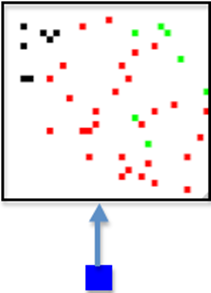
\includegraphics{img-19.png}
\end{figure}


\section{close\_display}
\label{5-Display/display:close-display}
If X display is enabled, then Rank 0 destroys the X Window and closes the display


\section{throttle}
\label{5-Display/display:throttle}
In order for better display, we wait between frames of animation.


\chapter{Core Functions}
\label{6-Core/core::doc}\label{6-Core/core:core-functions}

\section{move}
\label{6-Core/core:move}
If the person is not dead, then

\begin{Verbatim}[commandchars=\\\{\}]
        \PYG{k}{if}\PYG{p}{(}\PYG{n}{states}\PYG{p}{[}\PYG{n}{current\PYGZus{}person\PYGZus{}id}\PYG{p}{]} \PYG{o}{!}\PYG{o}{=} \PYG{n}{DEAD}\PYG{p}{)}
\end{Verbatim}

First, the function randomly picks whether the person moves left or right
or does not move in the x dimension.

The code uses (random() \% 3) - 1; to achieve this. (random() \% 3)
returns either 0, 1, or 2. Subtracting 1 from this produces -1, 0, or 1.
This means the person can move to the right, stay in place (0), or move
to the left (-1).

then the function randomly picks whether the person moves up or down or
does not move in the y dimension. This is similar to movement in x dimension.

\begin{Verbatim}[commandchars=\\\{\}]
            \PYG{c+c1}{// The thread randomly picks whether the person moves left }
            \PYG{c+c1}{// or right or does not move in the x dimension}
            \PYG{n}{x\PYGZus{}move\PYGZus{}direction} \PYG{o}{=} \PYG{p}{(}\PYG{n}{random}\PYG{p}{(}\PYG{p}{)} \PYG{o}{\PYGZpc{}} \PYG{l+m+mi}{3}\PYG{p}{)} \PYG{o}{-} \PYG{l+m+mi}{1}\PYG{p}{;}

            \PYG{c+c1}{// The thread randomly picks whether the person moves up}
            \PYG{c+c1}{// or down or does not move in the y dimension}
            \PYG{n}{y\PYGZus{}move\PYGZus{}direction} \PYG{o}{=} \PYG{p}{(}\PYG{n}{random}\PYG{p}{(}\PYG{p}{)} \PYG{o}{\PYGZpc{}} \PYG{l+m+mi}{3}\PYG{p}{)} \PYG{o}{-} \PYG{l+m+mi}{1}\PYG{p}{;}
\end{Verbatim}

Next, If the person will remain in the bounds of the environment after
moving, then

We check this by making sure the person’s x location is greater than or
equal to 0 and less than the width of the environment and that the
person’s y location is greater than or equal to 0 and less than the
height of the environment. In the code, it looks like this:

\begin{Verbatim}[commandchars=\\\{\}]
            \PYG{k}{if}\PYG{p}{(}\PYG{p}{(}\PYG{n}{x\PYGZus{}locations}\PYG{p}{[}\PYG{n}{current\PYGZus{}person\PYGZus{}id}\PYG{p}{]} \PYG{o}{+} \PYG{n}{x\PYGZus{}move\PYGZus{}direction} \PYG{o}{\PYGZgt{}}\PYG{o}{=} \PYG{l+m+mi}{0}\PYG{p}{)}
                \PYG{o}{\PYGZam{}}\PYG{o}{\PYGZam{}} \PYG{p}{(}\PYG{n}{x\PYGZus{}locations}\PYG{p}{[}\PYG{n}{current\PYGZus{}person\PYGZus{}id}\PYG{p}{]} 
                    \PYG{o}{+} \PYG{n}{x\PYGZus{}move\PYGZus{}direction} \PYG{o}{\PYGZlt{}} \PYG{n}{environment\PYGZus{}width}\PYG{p}{)}
                \PYG{o}{\PYGZam{}}\PYG{o}{\PYGZam{}} \PYG{p}{(}\PYG{n}{y\PYGZus{}locations}\PYG{p}{[}\PYG{n}{current\PYGZus{}person\PYGZus{}id}\PYG{p}{]} 
                    \PYG{o}{+} \PYG{n}{y\PYGZus{}move\PYGZus{}direction} \PYG{o}{\PYGZgt{}}\PYG{o}{=} \PYG{l+m+mi}{0}\PYG{p}{)}
                \PYG{o}{\PYGZam{}}\PYG{o}{\PYGZam{}} \PYG{p}{(}\PYG{n}{y\PYGZus{}locations}\PYG{p}{[}\PYG{n}{current\PYGZus{}person\PYGZus{}id}\PYG{p}{]} 
                    \PYG{o}{+} \PYG{n}{y\PYGZus{}move\PYGZus{}direction} \PYG{o}{\PYGZlt{}} \PYG{n}{environment\PYGZus{}height}\PYG{p}{)}\PYG{p}{)}
\end{Verbatim}

Finally, The function moves the person
\begin{figure}[htbp]
\centering

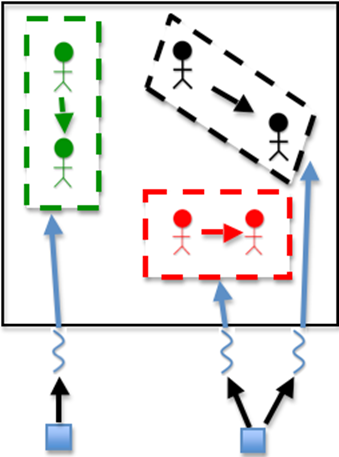
\includegraphics{img-20.png}
\end{figure}

\begin{Verbatim}[commandchars=\\\{\}]
                \PYG{n}{x\PYGZus{}locations}\PYG{p}{[}\PYG{n}{current\PYGZus{}person\PYGZus{}id}\PYG{p}{]} 
                \PYG{o}{+}\PYG{o}{=} \PYG{n}{x\PYGZus{}move\PYGZus{}direction}\PYG{p}{;}
                \PYG{n}{y\PYGZus{}locations}\PYG{p}{[}\PYG{n}{current\PYGZus{}person\PYGZus{}id}\PYG{p}{]} 
                \PYG{o}{+}\PYG{o}{=} \PYG{n}{y\PYGZus{}move\PYGZus{}direction}\PYG{p}{;}
\end{Verbatim}

The function is able to achieve this by simply changing values in the
\textbf{x\_locations} and \textbf{y\_locations} arrays.


\section{susceptible}
\label{6-Core/core:susceptible}
For each people, the function to do the following

\begin{Verbatim}[commandchars=\\\{\}]
    \PYG{k}{for}\PYG{p}{(}\PYG{n}{current\PYGZus{}person\PYGZus{}id} \PYG{o}{=} \PYG{l+m+mi}{0}\PYG{p}{;} \PYG{n}{current\PYGZus{}person\PYGZus{}id} 
        \PYG{o}{\PYGZlt{}}\PYG{o}{=} \PYG{n}{global}\PYG{o}{-}\PYG{o}{\PYGZgt{}}\PYG{n}{number\PYGZus{}of\PYGZus{}people} \PYG{o}{-} \PYG{l+m+mi}{1}\PYG{p}{;} \PYG{n}{current\PYGZus{}person\PYGZus{}id}\PYG{o}{+}\PYG{o}{+}\PYG{p}{)}
\end{Verbatim}

If the person is susceptible,

\begin{Verbatim}[commandchars=\\\{\}]
        \PYG{k}{if}\PYG{p}{(}\PYG{n}{states}\PYG{p}{[}\PYG{n}{current\PYGZus{}person\PYGZus{}id}\PYG{p}{]} \PYG{o}{=}\PYG{o}{=} \PYG{n}{SUSCEPTIBLE}\PYG{p}{)}
\end{Verbatim}

For each of the infected people or until the number of infected people nearby is 1, the function does the following

\begin{Verbatim}[commandchars=\\\{\}]
            \PYG{k}{for}\PYG{p}{(}\PYG{n}{my\PYGZus{}person} \PYG{o}{=} \PYG{l+m+mi}{0}\PYG{p}{;} \PYG{n}{my\PYGZus{}person} \PYG{o}{\PYGZlt{}}\PYG{o}{=} \PYG{n}{global}\PYG{o}{-}\PYG{o}{\PYGZgt{}}\PYG{n}{num\PYGZus{}infected} \PYG{o}{-} \PYG{l+m+mi}{1}
                \PYG{o}{\PYGZam{}}\PYG{o}{\PYGZam{}} \PYG{n}{num\PYGZus{}infected\PYGZus{}nearby} \PYG{o}{\PYGZlt{}} \PYG{l+m+mi}{1}\PYG{p}{;} \PYG{n}{my\PYGZus{}person}\PYG{o}{+}\PYG{o}{+}\PYG{p}{)}
\end{Verbatim}

If the person is within the infection radius, then

\begin{Verbatim}[commandchars=\\\{\}]
                \PYG{k}{if}\PYG{p}{(}\PYG{p}{(}\PYG{n}{x\PYGZus{}locations}\PYG{p}{[}\PYG{n}{current\PYGZus{}person\PYGZus{}id}\PYG{p}{]} 
                    \PYG{o}{\PYGZgt{}} \PYG{n}{infected\PYGZus{}x\PYGZus{}locations}\PYG{p}{[}\PYG{n}{my\PYGZus{}person}\PYG{p}{]} \PYG{o}{-} \PYG{n}{infection\PYGZus{}radius}\PYG{p}{)}
                    \PYG{o}{\PYGZam{}}\PYG{o}{\PYGZam{}} \PYG{p}{(}\PYG{n}{x\PYGZus{}locations}\PYG{p}{[}\PYG{n}{current\PYGZus{}person\PYGZus{}id}\PYG{p}{]} 
                        \PYG{o}{\PYGZlt{}} \PYG{n}{infected\PYGZus{}x\PYGZus{}locations}\PYG{p}{[}\PYG{n}{my\PYGZus{}person}\PYG{p}{]} \PYG{o}{+} \PYG{n}{infection\PYGZus{}radius}\PYG{p}{)}
                    \PYG{o}{\PYGZam{}}\PYG{o}{\PYGZam{}} \PYG{p}{(}\PYG{n}{y\PYGZus{}locations}\PYG{p}{[}\PYG{n}{current\PYGZus{}person\PYGZus{}id}\PYG{p}{]}
                        \PYG{o}{\PYGZgt{}} \PYG{n}{infected\PYGZus{}y\PYGZus{}locations}\PYG{p}{[}\PYG{n}{my\PYGZus{}person}\PYG{p}{]} \PYG{o}{-} \PYG{n}{infection\PYGZus{}radius}\PYG{p}{)}
                    \PYG{o}{\PYGZam{}}\PYG{o}{\PYGZam{}} \PYG{p}{(}\PYG{n}{y\PYGZus{}locations}\PYG{p}{[}\PYG{n}{current\PYGZus{}person\PYGZus{}id}\PYG{p}{]}
                        \PYG{o}{\PYGZlt{}} \PYG{n}{infected\PYGZus{}y\PYGZus{}locations}\PYG{p}{[}\PYG{n}{my\PYGZus{}person}\PYG{p}{]} \PYG{o}{+} \PYG{n}{infection\PYGZus{}radius}\PYG{p}{)}\PYG{p}{)}
\end{Verbatim}

Finally, the function increments the number of infected people nearby

\begin{Verbatim}[commandchars=\\\{\}]
                    \PYG{n}{num\PYGZus{}infected\PYGZus{}nearby}\PYG{o}{+}\PYG{o}{+}\PYG{p}{;}
\end{Verbatim}
\begin{figure}[htbp]
\centering

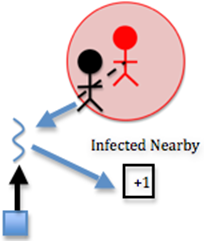
\includegraphics{img-21.png}
\end{figure}

This is where a large chunk of the algorithm’s computation occurs. Each
susceptible person must be computed with each infected person to
determine how many infected people are nearby each person. Two nested
loops means many computations. In this step, the computation is fairly
simple, however. The function simply increments the
\textbf{num\_infected\_nearby} variable.

Note in the code that if the number of infected nearby is greater than
or equal to 1 and we have \textbf{SHOW\_RESULTS} enabled, we increment the
\textbf{num\_infection\_attempts} variable. This helps us keep track of the
number of attempted infections, which will help us calculate the actual
contagiousness of the disease at the end of the simulation.

If there is at least one infected person nearby, and a random
number less than 100 is less than or equal to the contagiousness factor,
then

\begin{Verbatim}[commandchars=\\\{\}]
            \PYG{k}{if}\PYG{p}{(}\PYG{n}{num\PYGZus{}infected\PYGZus{}nearby} \PYG{o}{\PYGZgt{}}\PYG{o}{=} \PYG{l+m+mi}{1} \PYG{o}{\PYGZam{}}\PYG{o}{\PYGZam{}} \PYG{p}{(}\PYG{n}{random}\PYG{p}{(}\PYG{p}{)} \PYG{o}{\PYGZpc{}} \PYG{l+m+mi}{100}\PYG{p}{)} 
                \PYG{o}{\PYGZlt{}}\PYG{o}{=} \PYG{n}{contagiousness\PYGZus{}factor}\PYG{p}{)}
\end{Verbatim}

Recall that the contagiousness factor is the likelihood that the disease
will be spread. We measure this as a number less than 100. For example,
if there is a 30\% chance of contagiousness, we use 30 as the value of
the contagiousness factor. To figure out if the disease is spread for
any given interaction of people, we find a random number less than 100
and check if it is less than or equal to the contagiousness factor,
because this will be equivalent to calculating the odds of actually
spreading the disease (e.g. there is a 30\% chance of spreading the
disease and also a 30\% chance that a random number less than 100 will be
less than or equal to 30).

The function changes the state to infected

\begin{Verbatim}[commandchars=\\\{\}]
                \PYG{n}{states}\PYG{p}{[}\PYG{n}{current\PYGZus{}person\PYGZus{}id}\PYG{p}{]} \PYG{o}{=} \PYG{n}{INFECTED}\PYG{p}{;}
\end{Verbatim}

The function updates the counters

\begin{Verbatim}[commandchars=\\\{\}]
                \PYG{c+c1}{// The thread updates the counters}
                \PYG{n}{global}\PYG{o}{-}\PYG{o}{\PYGZgt{}}\PYG{n}{num\PYGZus{}infected}\PYG{o}{+}\PYG{o}{+}\PYG{p}{;}
                \PYG{n}{global}\PYG{o}{-}\PYG{o}{\PYGZgt{}}\PYG{n}{num\PYGZus{}susceptible}\PYG{o}{-}\PYG{o}{-}\PYG{p}{;}
\end{Verbatim}
\begin{figure}[htbp]
\centering

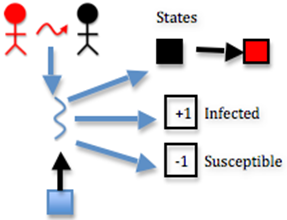
\includegraphics{img-22.png}
\end{figure}

These steps are as simple as updating the \textbf{states} array by
\textbf{states{[}my\_current\_person\_id{]} = INFECTED}, incrementing the
\textbf{num\_infected} variable, and decrementing the \textbf{num\_susceptible}
variable.

Note in the code that if the infection succeeds and we have
\textbf{SHOW\_RESULTS} enabled, we increment the \textbf{num\_infections variable}.
This helps us keep track of the actual number of infections, which will
help us calculate the actual contagiousness of the disease at the end of
the simulation.


\section{infected}
\label{6-Core/core:infected}
For each people, the function to do the following

\begin{Verbatim}[commandchars=\\\{\}]
    \PYG{k}{for}\PYG{p}{(}\PYG{n}{current\PYGZus{}person\PYGZus{}id} \PYG{o}{=} \PYG{l+m+mi}{0}\PYG{p}{;} \PYG{n}{current\PYGZus{}person\PYGZus{}id} 
        \PYG{o}{\PYGZlt{}}\PYG{o}{=} \PYG{n}{global}\PYG{o}{-}\PYG{o}{\PYGZgt{}}\PYG{n}{number\PYGZus{}of\PYGZus{}people} \PYG{o}{-} \PYG{l+m+mi}{1}\PYG{p}{;} \PYG{n}{current\PYGZus{}person\PYGZus{}id}\PYG{o}{+}\PYG{o}{+}\PYG{p}{)}
\end{Verbatim}

If the person is infected and has been for the full duration of the disease, then

\begin{Verbatim}[commandchars=\\\{\}]
        \PYG{k}{if}\PYG{p}{(}\PYG{n}{states}\PYG{p}{[}\PYG{n}{current\PYGZus{}person\PYGZus{}id}\PYG{p}{]} \PYG{o}{=}\PYG{o}{=} \PYG{n}{INFECTED}
            \PYG{o}{\PYGZam{}}\PYG{o}{\PYGZam{}} \PYG{n}{num\PYGZus{}days\PYGZus{}infected}\PYG{p}{[}\PYG{n}{current\PYGZus{}person\PYGZus{}id}\PYG{p}{]} 
            \PYG{o}{=}\PYG{o}{=} \PYG{n}{duration\PYGZus{}of\PYGZus{}disease}\PYG{p}{)}
\end{Verbatim}

Note in the code that if we have \textbf{SHOW\_RESULTS} enabled, we increment the
\textbf{num\_recovery\_attempts} variable. This helps us keep track of the
number of attempted recoveries, which will help us calculate the actual
deadliness of the disease at the end of the simulation.

\begin{Verbatim}[commandchars=\\\{\}]
            \PYG{n}{stats}\PYG{o}{-}\PYG{o}{\PYGZgt{}}\PYG{n}{num\PYGZus{}recovery\PYGZus{}attempts}\PYG{o}{+}\PYG{o}{+}\PYG{p}{;}
\end{Verbatim}

If a random number less than 100 is less than the deadliness factor, then

\begin{Verbatim}[commandchars=\\\{\}]
            \PYG{k}{if}\PYG{p}{(}\PYG{p}{(}\PYG{n}{random}\PYG{p}{(}\PYG{p}{)} \PYG{o}{\PYGZpc{}} \PYG{l+m+mi}{100}\PYG{p}{)} \PYG{o}{\PYGZlt{}} \PYG{n}{deadliness\PYGZus{}factor}\PYG{p}{)}
\end{Verbatim}

The function changes the person’s state to dead

\begin{Verbatim}[commandchars=\\\{\}]
                \PYG{n}{states}\PYG{p}{[}\PYG{n}{current\PYGZus{}person\PYGZus{}id}\PYG{p}{]} \PYG{o}{=} \PYG{n}{DEAD}\PYG{p}{;}
\end{Verbatim}

The function updates the counters

\begin{Verbatim}[commandchars=\\\{\}]
                \PYG{c+c1}{// The thread updates the counters}
                \PYG{n}{global}\PYG{o}{-}\PYG{o}{\PYGZgt{}}\PYG{n}{num\PYGZus{}dead}\PYG{o}{+}\PYG{o}{+}\PYG{p}{;}
                \PYG{n}{global}\PYG{o}{-}\PYG{o}{\PYGZgt{}}\PYG{n}{num\PYGZus{}infected}\PYG{o}{-}\PYG{o}{-}\PYG{p}{;}
\end{Verbatim}
\begin{figure}[htbp]
\centering

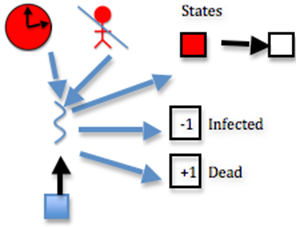
\includegraphics{img-23.png}
\end{figure}

This step is effectively the same as function susceptible, considering deadliness instead of contagiousness. The difference here is the following step:

Otherwise,

The function changes the person’s state to immune

\begin{Verbatim}[commandchars=\\\{\}]
                \PYG{n}{states}\PYG{p}{[}\PYG{n}{current\PYGZus{}person\PYGZus{}id}\PYG{p}{]} \PYG{o}{=} \PYG{n}{IMMUNE}\PYG{p}{;}
\end{Verbatim}

The function updates the counters

\begin{Verbatim}[commandchars=\\\{\}]
                \PYG{c+c1}{// The thread updates the counters}
                \PYG{n}{global}\PYG{o}{-}\PYG{o}{\PYGZgt{}}\PYG{n}{num\PYGZus{}immune}\PYG{o}{+}\PYG{o}{+}\PYG{p}{;}
                \PYG{n}{global}\PYG{o}{-}\PYG{o}{\PYGZgt{}}\PYG{n}{num\PYGZus{}infected}\PYG{o}{-}\PYG{o}{-}\PYG{p}{;}
\end{Verbatim}
\begin{figure}[htbp]
\centering

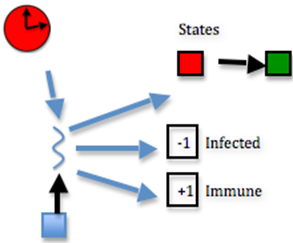
\includegraphics{img-24.png}
\end{figure}

If deadliness fails, then immunity succeeds.

Note in the code that if the person dies and we have \textbf{SHOW\_RESULTS}
enabled, we increment the \textbf{num\_deaths} variable. This helps us keep
track of the actual number of deaths, which will help us calculate the
actual deadliness of the disease at the end of the simulation.

\begin{Verbatim}[commandchars=\\\{\}]
                \PYG{c+c1}{// The thread updates stats counter}
                \PYG{c+cp}{\PYGZsh{}}\PYG{c+cp}{ifdef SHOW\PYGZus{}RESULTS}
                    \PYG{n}{stats}\PYG{o}{-}\PYG{o}{\PYGZgt{}}\PYG{n}{num\PYGZus{}deaths}\PYG{o}{+}\PYG{o}{+}\PYG{p}{;}
                \PYG{c+cp}{\PYGZsh{}}\PYG{c+cp}{endif}
\end{Verbatim}


\section{update\_days\_infected}
\label{6-Core/core:update-days-infected}
For each people, the function to do the following

\begin{Verbatim}[commandchars=\\\{\}]
    \PYG{k}{for}\PYG{p}{(}\PYG{n}{current\PYGZus{}person\PYGZus{}id} \PYG{o}{=} \PYG{l+m+mi}{0}\PYG{p}{;} \PYG{n}{current\PYGZus{}person\PYGZus{}id} 
        \PYG{o}{\PYGZlt{}}\PYG{o}{=} \PYG{n}{global}\PYG{o}{-}\PYG{o}{\PYGZgt{}}\PYG{n}{number\PYGZus{}of\PYGZus{}people} \PYG{o}{-} \PYG{l+m+mi}{1}\PYG{p}{;} \PYG{n}{current\PYGZus{}person\PYGZus{}id}\PYG{o}{+}\PYG{o}{+}\PYG{p}{)}
\end{Verbatim}

If the person is infected, then

\begin{Verbatim}[commandchars=\\\{\}]
        \PYG{k}{if}\PYG{p}{(}\PYG{n}{states}\PYG{p}{[}\PYG{n}{current\PYGZus{}person\PYGZus{}id}\PYG{p}{]} \PYG{o}{=}\PYG{o}{=} \PYG{n}{INFECTED}\PYG{p}{)}
\end{Verbatim}

Increment the number of days the person has been infected

\begin{Verbatim}[commandchars=\\\{\}]
            \PYG{n}{num\PYGZus{}days\PYGZus{}infected}\PYG{p}{[}\PYG{n}{current\PYGZus{}person\PYGZus{}id}\PYG{p}{]}\PYG{o}{+}\PYG{o}{+}\PYG{p}{;}
\end{Verbatim}
\begin{figure}[htbp]
\centering

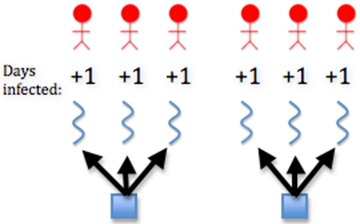
\includegraphics{img-25.png}
\end{figure}

This is achieved by incrementing each member of the
\textbf{num\_days\_infected} array, which can be done as follows:
\textbf{num\_days\_infected{[}my\_current\_person\_id{]}++}


\chapter{Finish Functions}
\label{7-Finalize/finalize:finish-functions}\label{7-Finalize/finalize::doc}

\section{show\_results}
\label{7-Finalize/finalize:show-results}
At the end of the code, if we are choosing to show results, we print out
the final counts of susceptible, infected, immune, and dead people. We
also print the actual contagiousness and actual deadliness of the
disease. To perform these two calculations, we use the following code
(using the contagiousness as the example):

\begin{Verbatim}[commandchars=\\\{\}]
		\PYG{l+m+mf}{100.0} \PYG{o}{*} \PYG{p}{(}\PYG{n}{stats}\PYG{o}{-}\PYG{o}{\PYGZgt{}}\PYG{n}{num\PYGZus{}infections} \PYG{o}{/} \PYG{p}{(}\PYG{n}{stats}\PYG{o}{-}\PYG{o}{\PYGZgt{}}\PYG{n}{num\PYGZus{}infection\PYGZus{}attempts} 
			\PYG{o}{=}\PYG{o}{=} \PYG{l+m+mi}{0} \PYG{o}{?} \PYG{l+m+mi}{1} \PYG{o}{:} \PYG{n}{stats}\PYG{o}{-}\PYG{o}{\PYGZgt{}}\PYG{n}{num\PYGZus{}infection\PYGZus{}attempts}\PYG{p}{)}\PYG{p}{)}\PYG{p}{,} 
		\PYG{l+m+mf}{100.0} \PYG{o}{*} \PYG{p}{(}\PYG{n}{stats}\PYG{o}{-}\PYG{o}{\PYGZgt{}}\PYG{n}{num\PYGZus{}deaths} \PYG{o}{/} \PYG{p}{(}\PYG{n}{stats}\PYG{o}{-}\PYG{o}{\PYGZgt{}}\PYG{n}{num\PYGZus{}recovery\PYGZus{}attempts} 
			\PYG{o}{=}\PYG{o}{=} \PYG{l+m+mi}{0} \PYG{o}{?} \PYG{l+m+mi}{1} \PYG{o}{:} \PYG{n}{stats}\PYG{o}{-}\PYG{o}{\PYGZgt{}}\PYG{n}{num\PYGZus{}recovery\PYGZus{}attempts}\PYG{p}{)}\PYG{p}{)}\PYG{p}{)}\PYG{p}{;}
\end{Verbatim}

In this code, the ternary operators (? and :) are used to return one
value if something is true and another value if it isn’t. The thing we
are checking for truth is \textbf{num\_infection\_attempts == 0}. If this is
true, i.e. if we didn’t attempt any infection attempts at all, then we
say there was actually 1 infection attempt (this is to avoid a divide by
zero error). Otherwise, we return the actual number of infection
attempts. This value becomes the dividend for \textbf{num\_infections}; in
other words, we divide the number of actual infections by the number of
total infections. This will give us a value less than 1, so we multiply
it by 100 to obtain the actual contagiousness factor of the disease. A
similar procedure is performed to calculate the actual deadliness
factor.


\section{cleanup}
\label{7-Finalize/finalize:cleanup}
If X display is enabled, then Rank 0 destroys the X Window and closes the display

\begin{Verbatim}[commandchars=\\\{\}]
    \PYG{n}{close\PYGZus{}display}\PYG{p}{(}\PYG{n}{dpy}\PYG{p}{)}\PYG{p}{;}
\end{Verbatim}

Since we allocated arrays dynamically, we need to release them back
to the heap using the \textbf{free} function. We do this in the reverse order
than we used \textbf{malloc}, so \textbf{environment} will come first and \textbf{x\_locations}
will come last.

\begin{Verbatim}[commandchars=\\\{\}]
    \PYG{c+c1}{// free text display environment}
	\PYG{c+cp}{\PYGZsh{}}\PYG{c+cp}{ifdef TEXT\PYGZus{}DISPLAY }
	\PYG{k+kt}{int} \PYG{n}{current\PYGZus{}location\PYGZus{}x}\PYG{p}{;}
	\PYG{k}{for}\PYG{p}{(}\PYG{n}{current\PYGZus{}location\PYGZus{}x} \PYG{o}{=} \PYG{n}{constant}\PYG{o}{-}\PYG{o}{\PYGZgt{}}\PYG{n}{environment\PYGZus{}width} \PYG{o}{-} \PYG{l+m+mi}{1}\PYG{p}{;} 
		\PYG{n}{current\PYGZus{}location\PYGZus{}x} \PYG{o}{\PYGZgt{}}\PYG{o}{=} \PYG{l+m+mi}{0}\PYG{p}{;} \PYG{n}{current\PYGZus{}location\PYGZus{}x}\PYG{o}{-}\PYG{o}{-}\PYG{p}{)}
	\PYG{p}{\PYGZob{}}
		\PYG{n}{free}\PYG{p}{(}\PYG{n}{dpy}\PYG{o}{-}\PYG{o}{\PYGZgt{}}\PYG{n}{environment}\PYG{p}{[}\PYG{n}{current\PYGZus{}location\PYGZus{}x}\PYG{p}{]}\PYG{p}{)}\PYG{p}{;}
	\PYG{p}{\PYGZcb{}}
	\PYG{n}{free}\PYG{p}{(}\PYG{n}{dpy}\PYG{o}{-}\PYG{o}{\PYGZgt{}}\PYG{n}{environment}\PYG{p}{)}\PYG{p}{;}
	\PYG{c+cp}{\PYGZsh{}}\PYG{c+cp}{endif}

	\PYG{c+c1}{// free arrays allocated in global struct}
	\PYG{n}{free}\PYG{p}{(}\PYG{n}{global}\PYG{o}{-}\PYG{o}{\PYGZgt{}}\PYG{n}{x\PYGZus{}locations}\PYG{p}{)}\PYG{p}{;}
	\PYG{n}{free}\PYG{p}{(}\PYG{n}{global}\PYG{o}{-}\PYG{o}{\PYGZgt{}}\PYG{n}{y\PYGZus{}locations}\PYG{p}{)}\PYG{p}{;}
	\PYG{n}{free}\PYG{p}{(}\PYG{n}{global}\PYG{o}{-}\PYG{o}{\PYGZgt{}}\PYG{n}{infected\PYGZus{}y\PYGZus{}locations}\PYG{p}{)}\PYG{p}{;}
	\PYG{n}{free}\PYG{p}{(}\PYG{n}{global}\PYG{o}{-}\PYG{o}{\PYGZgt{}}\PYG{n}{infected\PYGZus{}x\PYGZus{}locations}\PYG{p}{)}\PYG{p}{;}
	\PYG{n}{free}\PYG{p}{(}\PYG{n}{global}\PYG{o}{-}\PYG{o}{\PYGZgt{}}\PYG{n}{states}\PYG{p}{)}\PYG{p}{;}
	\PYG{n}{free}\PYG{p}{(}\PYG{n}{global}\PYG{o}{-}\PYG{o}{\PYGZgt{}}\PYG{n}{num\PYGZus{}days\PYGZus{}infected}\PYG{p}{)}\PYG{p}{;}
\end{Verbatim}


\chapter{Build and Run}
\label{7.1-BuildAndRun/build::doc}\label{7.1-BuildAndRun/build:build-and-run}
When you create the executable for this program, you will need to set some flags that are particular for your machine, particularly if you want to run it with the graphical display, which uses the X11 library.  This should work on linux machines and Mac OS X machines that have X11 installed.

Lines 12-14 in the Makefile, shown below and included with the code, are where you set paths to the X11 library and include directories.  On some linux machines you may not need to set either of these, which is why they are commented out.

If you want to use a text display instead of the graphical X11 display, uncomment line 20 and comment line 22.  When rigging the code to test for performance, you might want to eliminate the display of each iteration completely, in which case you can comment line 20 and 22.

\begin{Verbatim}[commandchars=\\\{\},numbers=left,firstnumber=1,stepnumber=1]
\PYG{c}{\PYGZsh{} DESCRIPTION:  Makefile for serial code in C}
\PYG{c}{\PYGZsh{} AUTHOR:       Yu Zhao, Macalester College}
\PYG{c}{\PYGZsh{} DATE:         Original for Area Under A Curve module, September, 2011.}
\PYG{c}{\PYGZsh{}	Modified for Infectious Disease module, November, 2011. by Aaron Weedon}
\PYG{c}{\PYGZsh{}	Modified for Infectious Disease module, July, 2013, by Yu Zhao}

\PYG{c}{\PYGZsh{} Code prefix}
\PYG{n+nv}{PROGRAM\PYGZus{}PREFIX}\PYG{o}{=}Pandemic

\PYG{c}{\PYGZsh{} Compilers and flags}
\PYG{n+nv}{CC}\PYG{o}{=}gcc
\PYG{c}{\PYGZsh{}XLIB\PYGZus{}LOC=/opt/X11/lib    \PYGZsh{}Mac OS X XQuartz installed here}
\PYG{c}{\PYGZsh{}XLIB\PYGZus{}LOC=/usr/X11R6/lib   \PYGZsh{}some unix systems may have this}
\PYG{c}{\PYGZsh{}XLIB\PYGZus{}INC=/opt/X11/include}

ifdef ICC
	\PYG{n+nv}{CC}\PYG{o}{=}icc
endif

\PYG{c}{\PYGZsh{}CFLAGS+=-DTEXT\PYGZus{}DISPLAY \PYGZsh{} Uncomment to show text display}

CFLAGS+\PYG{o}{=}-DX\PYGZus{}DISPLAY -I \PYG{k}{\PYGZdl{}(}XLIB\PYGZus{}INC\PYG{k}{)} -L\PYG{k}{\PYGZdl{}(}XLIB\PYGZus{}LOC\PYG{k}{)} -lX11 \PYG{c}{\PYGZsh{} Uncomment to show X display}

CFLAGS+\PYG{o}{=}-DSHOW\PYGZus{}RESULTS \PYG{c}{\PYGZsh{} Uncomment to make the program print its results}

\PYG{c}{\PYGZsh{} Source files}
\PYG{n+nv}{SRCS}\PYG{o}{=}\PYG{k}{\PYGZdl{}(}PROGRAM\PYGZus{}PREFIX\PYG{k}{)}.c

\PYG{c}{\PYGZsh{} Make targets}
all: \PYG{k}{\PYGZdl{}(}PROGRAM\PYGZus{}PREFIX\PYG{k}{)}-serial

clean: 
	rm -f \PYG{k}{\PYGZdl{}(}PROGRAM\PYGZus{}PREFIX\PYG{k}{)}-serial

run:
	./\PYG{k}{\PYGZdl{}(}PROGRAM\PYGZus{}PREFIX\PYG{k}{)}-serial

\PYG{c}{\PYGZsh{} Make rules}
\PYG{k}{\PYGZdl{}(}PROGRAM\PYGZus{}PREFIX\PYG{k}{)}-serial: \PYG{k}{\PYGZdl{}(}SRCS\PYG{k}{)}
	\PYG{k}{\PYGZdl{}(}CC\PYG{k}{)} -o \PYG{k}{\PYGZdl{}(}PROGRAM\PYGZus{}PREFIX\PYG{k}{)}-serial \PYG{k}{\PYGZdl{}(}SRCS\PYG{k}{)} \PYG{k}{\PYGZdl{}(}CFLAGS\PYG{k}{)} 

\PYG{k}{\PYGZdl{}(}SRCS\PYG{k}{)}: Core.h Defaults.h Display.h Finalize.h Infection.h Initialize.h
\end{Verbatim}


\section{Build}
\label{7.1-BuildAndRun/build:build}
\begin{Verbatim}[commandchars=\\\{\}]
\PYG{n}{make}
\end{Verbatim}


\section{Run}
\label{7.1-BuildAndRun/build:run}
\begin{Verbatim}[commandchars=\\\{\}]
./Pandemic-serial
\end{Verbatim}

The default values start with a simulation of approximately 50 people.

To see what elements of the computation you can change, try this:

\begin{Verbatim}[commandchars=\\\{\}]
./Pandemic-serial -?
\end{Verbatim}

It should give you something like this:

\begin{Verbatim}[commandchars=\\\{\}]
./Pandemic-serial: illegal option -- ?

Usage: ./Pandemic-serial [-n number\_of\_people][-i num\_initially\_infected
[-w environment\_width][-h environment\_height][-t total\_number\_of\_days]
[-T duration\_of\_disease][-c contagiousness\_factor][-d infection\_radius]
[-D deadliness\_factor][-m microseconds\_per\_day]
\end{Verbatim}

Note that these are defined and set in the \emph{parse\_args()} function in Initialize.h.

If you comment out lines 20 and 22 of the Makefile shown above, you can try getting some preliminary basic sense of how fast the program runs with various sizes of the problem (in this case the number of people).  First, comment lines 20 and 22 in the Makefile and do the following:

\begin{Verbatim}[commandchars=\\\{\}]
make clean
make
\end{Verbatim}

Then execute various problem sizes, taking no time between iterations, as follows:

\begin{Verbatim}[commandchars=\\\{\}]
time ./Pandemic-serial -n 20000 -m 0
\end{Verbatim}

Experiment by changing the value of n higher and lower.  You should see the program take more time as you increase the number of people.  Experiment with some of the other parameters also. Do some investigation of what the unix time command does.  This is a very rough way to see how fast your program runs.  There are preferable ways to instrument the code itself that you could investigate.


\chapter{Including OpenMP}
\label{8-OpenMP/openmp:including-openmp}\label{8-OpenMP/openmp::doc}
\code{Download Pandemic-OMP.tgz}

It is really easy to include OpenMP features into existing code we have. All we need to do is to identify all the functions that could use OpenMP. There are in total 5 functions that could use OpenMP to increase performance. The first function is the \textbf{init\_array()} function in \emph{Initialize.h} file. The next four functions are all the core functions inside \emph{Core.h} file.


\section{In Initialize.h}
\label{8-OpenMP/openmp:in-initialize-h}

\subsection{init\_array()}
\label{8-OpenMP/openmp:init-array}
This function can be divided into four parts: the first part sets the states of the initially infected people and sets the count of infected people. The second part sets states of the rest of the people and sets the of susceptible people. The third part sets random x and y locations for each people. The last part initilize the number of days infected of each people to 0.

Normally, to include OpenMP, all we need is to put \textbf{\#pragma omp parallel} in front of each of the for loops. However, our case is a little tricky. The problem is that we are reducing two counters in the first two parts of the function. Different from most parallel structure, reduction in OpenMP is pretty easy to implement. We just need to add a reduction literal,

\begin{Verbatim}[commandchars=\\\{\}]
    \PYG{c+cp}{\PYGZsh{}}\PYG{c+cp}{pragma omp parallel for private(current\PYGZus{}person\PYGZus{}id) \PYGZbs{}}
\PYG{c+cp}{        reduction(+:num\PYGZus{}infected\PYGZus{}local)}
\end{Verbatim}

The problem lies on that the counters we are reducing is inside a structure, namely, the global structure. OpenMP does not support reduction to structures. Therefore, we solve this problem by first create local instance such as \textbf{num\_infected\_local} that equals to counter \textbf{num\_infected} in global struct

\begin{Verbatim}[commandchars=\\\{\}]
    \PYG{k+kt}{int} \PYG{n}{num\PYGZus{}infected\PYGZus{}local} \PYG{o}{=} \PYG{n}{global}\PYG{o}{-}\PYG{o}{\PYGZgt{}}\PYG{n}{num\PYGZus{}infected}\PYG{p}{;}
\end{Verbatim}

we can then, reduce to local instance,

\begin{Verbatim}[commandchars=\\\{\}]
        \PYG{n}{num\PYGZus{}infected\PYGZus{}local}\PYG{o}{+}\PYG{o}{+}\PYG{p}{;}
\end{Verbatim}

Finally, we put local instance back to struct.

\begin{Verbatim}[commandchars=\\\{\}]
    \PYG{n}{global}\PYG{o}{-}\PYG{o}{\PYGZgt{}}\PYG{n}{num\PYGZus{}infected} \PYG{o}{=} \PYG{n}{num\PYGZus{}infected\PYGZus{}local}\PYG{p}{;}
\end{Verbatim}

We then use the same reduction method for the second part of the function. The third and Fourth part of the function does not reduce any counters, which means we don't need worry about reduction at all.


\section{In Core.h}
\label{8-OpenMP/openmp:in-core-h}
There are four core functions inside \emph{Core.h} file, and all of them can be parallelized using OpenMP.


\subsection{move()}
\label{8-OpenMP/openmp:move}
This function is easy to parallelize because it does not perform any reduction. However, we need to specify the variables that is private to each OpenMP threads. \textbf{current\_person\_id} is iterator that is clearly private. \textbf{x\_move\_direction} and \textbf{y\_move\_direction} are different for every thread, which means they are private as well.

\begin{Verbatim}[commandchars=\\\{\}]
    \PYG{c+cp}{\PYGZsh{}}\PYG{c+cp}{ifdef \PYGZus{}OPENMP}
    \PYG{c+cp}{\PYGZsh{}}\PYG{c+cp}{pragma omp parallel for private(current\PYGZus{}person\PYGZus{}id, x\PYGZus{}move\PYGZus{}direction, \PYGZbs{}}
\PYG{c+cp}{        y\PYGZus{}move\PYGZus{}direction)}
    \PYG{c+cp}{\PYGZsh{}}\PYG{c+cp}{endif }
\end{Verbatim}


\subsection{susceptible()}
\label{8-OpenMP/openmp:susceptible}
This function is relatively hard to parallelize because it has four counters to reduce. Luckily, we already developed our way of reducing counters in \textbf{init\_array()} function, which means we can use same method in here.

Creating local instances

\begin{Verbatim}[commandchars=\\\{\}]
    \PYG{c+c1}{// OMP does not support reduction to struct, create local instance}
    \PYG{c+c1}{// and then put local instance back to struct}
    \PYG{k+kt}{int} \PYG{n}{num\PYGZus{}infection\PYGZus{}attempts\PYGZus{}local} \PYG{o}{=} \PYG{n}{stats}\PYG{o}{-}\PYG{o}{\PYGZgt{}}\PYG{n}{num\PYGZus{}infection\PYGZus{}attempts}\PYG{p}{;}
    \PYG{k+kt}{int} \PYG{n}{num\PYGZus{}infections\PYGZus{}local} \PYG{o}{=} \PYG{n}{stats}\PYG{o}{-}\PYG{o}{\PYGZgt{}}\PYG{n}{num\PYGZus{}infections}\PYG{p}{;}
    \PYG{k+kt}{int} \PYG{n}{num\PYGZus{}infected\PYGZus{}local} \PYG{o}{=} \PYG{n}{global}\PYG{o}{-}\PYG{o}{\PYGZgt{}}\PYG{n}{num\PYGZus{}infected}\PYG{p}{;}
    \PYG{k+kt}{int} \PYG{n}{num\PYGZus{}susceptible\PYGZus{}local} \PYG{o}{=} \PYG{n}{global}\PYG{o}{-}\PYG{o}{\PYGZgt{}}\PYG{n}{num\PYGZus{}susceptible}\PYG{p}{;}
\end{Verbatim}

OpenMP initialization

\begin{Verbatim}[commandchars=\\\{\}]
    \PYG{c+cp}{\PYGZsh{}}\PYG{c+cp}{ifdef \PYGZus{}OPENMP}
    \PYG{c+cp}{\PYGZsh{}}\PYG{c+cp}{pragma omp parallel for private(current\PYGZus{}person\PYGZus{}id, num\PYGZus{}infected\PYGZus{}nearby, \PYGZbs{}}
\PYG{c+cp}{        my\PYGZus{}person) reduction(+:num\PYGZus{}infection\PYGZus{}attempts\PYGZus{}local) \PYGZbs{}}
\PYG{c+cp}{        reduction(+:num\PYGZus{}infected\PYGZus{}local) reduction(+:num\PYGZus{}susceptible\PYGZus{}local) \PYGZbs{}}
\PYG{c+cp}{        reduction(+:num\PYGZus{}infections\PYGZus{}local)}
    \PYG{c+cp}{\PYGZsh{}}\PYG{c+cp}{endif }
\end{Verbatim}

Put local instances back to global struct

\begin{Verbatim}[commandchars=\\\{\}]
    \PYG{c+c1}{// update struct data with local instances}
    \PYG{n}{stats}\PYG{o}{-}\PYG{o}{\PYGZgt{}}\PYG{n}{num\PYGZus{}infection\PYGZus{}attempts} \PYG{o}{=} \PYG{n}{num\PYGZus{}infection\PYGZus{}attempts\PYGZus{}local}\PYG{p}{;}
    \PYG{n}{stats}\PYG{o}{-}\PYG{o}{\PYGZgt{}}\PYG{n}{num\PYGZus{}infections} \PYG{o}{=} \PYG{n}{num\PYGZus{}infections\PYGZus{}local}\PYG{p}{;}
    \PYG{n}{global}\PYG{o}{-}\PYG{o}{\PYGZgt{}}\PYG{n}{num\PYGZus{}infected} \PYG{o}{=} \PYG{n}{num\PYGZus{}infected\PYGZus{}local}\PYG{p}{;}
    \PYG{n}{global}\PYG{o}{-}\PYG{o}{\PYGZgt{}}\PYG{n}{num\PYGZus{}susceptible} \PYG{o}{=} \PYG{n}{num\PYGZus{}susceptible\PYGZus{}local}\PYG{p}{;}
\end{Verbatim}


\subsection{infected()}
\label{8-OpenMP/openmp:infected}
Similar to \textbf{susceptible()} function, we have five counters to reduce in this function.

Creating local instances

\begin{Verbatim}[commandchars=\\\{\}]
    \PYG{c+c1}{// OMP does not support reduction to struct, create local instance}
    \PYG{c+c1}{// and then put local instance back to struct}
    \PYG{k+kt}{int} \PYG{n}{num\PYGZus{}recovery\PYGZus{}attempts\PYGZus{}local} \PYG{o}{=} \PYG{n}{stats}\PYG{o}{-}\PYG{o}{\PYGZgt{}}\PYG{n}{num\PYGZus{}recovery\PYGZus{}attempts}\PYG{p}{;}
    \PYG{k+kt}{int} \PYG{n}{num\PYGZus{}deaths\PYGZus{}local} \PYG{o}{=} \PYG{n}{stats}\PYG{o}{-}\PYG{o}{\PYGZgt{}}\PYG{n}{num\PYGZus{}deaths}\PYG{p}{;}
    \PYG{k+kt}{int} \PYG{n}{num\PYGZus{}dead\PYGZus{}local} \PYG{o}{=} \PYG{n}{global}\PYG{o}{-}\PYG{o}{\PYGZgt{}}\PYG{n}{num\PYGZus{}dead}\PYG{p}{;}
    \PYG{k+kt}{int} \PYG{n}{num\PYGZus{}infected\PYGZus{}local} \PYG{o}{=} \PYG{n}{global}\PYG{o}{-}\PYG{o}{\PYGZgt{}}\PYG{n}{num\PYGZus{}infected}\PYG{p}{;}
    \PYG{k+kt}{int} \PYG{n}{num\PYGZus{}immune\PYGZus{}local} \PYG{o}{=} \PYG{n}{global}\PYG{o}{-}\PYG{o}{\PYGZgt{}}\PYG{n}{num\PYGZus{}immune}\PYG{p}{;}
\end{Verbatim}

OpenMP initialization

\begin{Verbatim}[commandchars=\\\{\}]
    \PYG{c+cp}{\PYGZsh{}}\PYG{c+cp}{ifdef \PYGZus{}OPENMP}
    \PYG{c+cp}{\PYGZsh{}}\PYG{c+cp}{pragma omp parallel for private(current\PYGZus{}person\PYGZus{}id) \PYGZbs{}}
\PYG{c+cp}{        reduction(+:num\PYGZus{}recovery\PYGZus{}attempts\PYGZus{}local) reduction(+:num\PYGZus{}dead\PYGZus{}local) \PYGZbs{}}
\PYG{c+cp}{        reduction(+:num\PYGZus{}infected\PYGZus{}local) reduction(+:num\PYGZus{}deaths\PYGZus{}local) \PYGZbs{}}
\PYG{c+cp}{        reduction(+:num\PYGZus{}immune\PYGZus{}local)}
    \PYG{c+cp}{\PYGZsh{}}\PYG{c+cp}{endif }
\end{Verbatim}

Put local instances back to global struct

\begin{Verbatim}[commandchars=\\\{\}]
    \PYG{c+c1}{// update struct data with local instances}
    \PYG{n}{stats}\PYG{o}{-}\PYG{o}{\PYGZgt{}}\PYG{n}{num\PYGZus{}recovery\PYGZus{}attempts} \PYG{o}{=} \PYG{n}{num\PYGZus{}recovery\PYGZus{}attempts\PYGZus{}local}\PYG{p}{;}
    \PYG{n}{stats}\PYG{o}{-}\PYG{o}{\PYGZgt{}}\PYG{n}{num\PYGZus{}deaths} \PYG{o}{=} \PYG{n}{num\PYGZus{}deaths\PYGZus{}local}\PYG{p}{;}
    \PYG{n}{global}\PYG{o}{-}\PYG{o}{\PYGZgt{}}\PYG{n}{num\PYGZus{}dead} \PYG{o}{=} \PYG{n}{num\PYGZus{}dead\PYGZus{}local}\PYG{p}{;}
    \PYG{n}{global}\PYG{o}{-}\PYG{o}{\PYGZgt{}}\PYG{n}{num\PYGZus{}infected} \PYG{o}{=} \PYG{n}{num\PYGZus{}infected\PYGZus{}local}\PYG{p}{;}
    \PYG{n}{global}\PYG{o}{-}\PYG{o}{\PYGZgt{}}\PYG{n}{num\PYGZus{}immune} \PYG{o}{=} \PYG{n}{num\PYGZus{}immune\PYGZus{}local}\PYG{p}{;}
\end{Verbatim}


\subsection{update\_days\_infected()}
\label{8-OpenMP/openmp:update-days-infected}
We don't have any reduction in this function, which means that the parallelization is relatively easy.

\begin{Verbatim}[commandchars=\\\{\}]
    \PYG{c+cp}{\PYGZsh{}}\PYG{c+cp}{ifdef \PYGZus{}OPENMP }
        \PYG{c+cp}{\PYGZsh{}}\PYG{c+cp}{pragma omp parallel for private(current\PYGZus{}person\PYGZus{}id)}
    \PYG{c+cp}{\PYGZsh{}}\PYG{c+cp}{endif}
\end{Verbatim}


\chapter{Build and Run the Parallel Version}
\label{8.1-ompBuildAndRun/omp_build::doc}\label{8.1-ompBuildAndRun/omp_build:build-and-run-the-parallel-version}
When you create the executable for this program, you will need to set some flags that are particular for your machine, particularly if you want to run it with the graphical display, which uses the X11 library.  This should work on linux machines and Mac OS X machines that have X11 installed.

Lines 12-14 in the Makefile, shown below and included with the code, are where you set paths to the X11 library and include directories.  On some linux machines you may not need to set either of these, which is why they are commented out.

In this case, lines 20 and 22 are commented because rather than seeing the display, we want to start looking at how the parallel code runs (real code wouldn't use the display for simulation modeling).  When rigging the code to test for performance, you really want to eliminate most of the output, so we have just left line 24 uncommented to see the final statistics after the whole simulation is completed.

\begin{Verbatim}[commandchars=\\\{\},numbers=left,firstnumber=1,stepnumber=1]
\PYG{c}{\PYGZsh{} DESCRIPTION:  Makefile for OpenMP code in C}
\PYG{c}{\PYGZsh{} AUTHOR:       Yu Zhao, Macalester College}
\PYG{c}{\PYGZsh{} DATE:         Original for Area Under A Curve module, September, 2011.}
\PYG{c}{\PYGZsh{}		Modified for Infectious Disease module, November, 2011. by Aaron Weedon}
\PYG{c}{\PYGZsh{}		Modified for Infectious Disease module, July, 2013, by Yu Zhao}

\PYG{c}{\PYGZsh{} Code prefix}
\PYG{n+nv}{PROGRAM\PYGZus{}PREFIX}\PYG{o}{=}Pandemic

\PYG{c}{\PYGZsh{} Compilers and flags}
\PYG{n+nv}{CC}\PYG{o}{=}gcc
\PYG{n+nv}{XLIB\PYGZus{}LOC}\PYG{o}{=}/opt/X11/lib    \PYG{c}{\PYGZsh{}Mac OS X XQuartz installed here}
\PYG{c}{\PYGZsh{}XLIB\PYGZus{}LOC=/usr/X11R6/lib   \PYGZsh{}some unix systems may have this}
\PYG{n+nv}{XLIB\PYGZus{}INC}\PYG{o}{=}/opt/X11/include    \PYG{c}{\PYGZsh{}Mac OS X XQuartz installed here}


\PYG{c}{\PYGZsh{} OpenMP}
\PYG{n+nv}{OPENMP\PYGZus{}FLAGS}\PYG{o}{=}-fopenmp

\PYG{c}{\PYGZsh{}CFLAGS+=-DTEXT\PYGZus{}DISPLAY \PYGZsh{} Uncomment to show text display}

\PYG{c}{\PYGZsh{}CFLAGS+=-DX\PYGZus{}DISPLAY -I \PYGZdl{}(XLIB\PYGZus{}INC) -L\PYGZdl{}(XLIB\PYGZus{}LOC) -lX11 \PYGZsh{} Uncomment to show X display}

CFLAGS+\PYG{o}{=}-DSHOW\PYGZus{}RESULTS \PYG{c}{\PYGZsh{} Uncomment to make the program print its results}

\PYG{c}{\PYGZsh{} Source files}
\PYG{n+nv}{SRCS}\PYG{o}{=}\PYG{k}{\PYGZdl{}(}PROGRAM\PYGZus{}PREFIX\PYG{k}{)}.c 

\PYG{c}{\PYGZsh{} Make targets}
all: \PYG{k}{\PYGZdl{}(}PROGRAM\PYGZus{}PREFIX\PYG{k}{)}-openmp

clean: 
	rm -f \PYG{k}{\PYGZdl{}(}PROGRAM\PYGZus{}PREFIX\PYG{k}{)}-openmp

run:
	./\PYG{k}{\PYGZdl{}(}PROGRAM\PYGZus{}PREFIX\PYG{k}{)}.c-openmp

\PYG{c}{\PYGZsh{} Make rules}
\PYG{k}{\PYGZdl{}(}PROGRAM\PYGZus{}PREFIX\PYG{k}{)}-openmp: \PYG{k}{\PYGZdl{}(}SRCS\PYG{k}{)}
	\PYG{k}{\PYGZdl{}(}CC\PYG{k}{)} -o \PYG{k}{\PYGZdl{}(}PROGRAM\PYGZus{}PREFIX\PYG{k}{)}-openmp \PYG{k}{\PYGZdl{}(}SRCS\PYG{k}{)} \PYG{k}{\PYGZdl{}(}OPENMP\PYGZus{}FLAGS\PYG{k}{)} \PYG{k}{\PYGZdl{}(}CFLAGS\PYG{k}{)}

\PYG{k}{\PYGZdl{}(}SRCS\PYG{k}{)}: Core.h Defaults.h Display.h Finalize.h Infection.h Initialize.h
\end{Verbatim}


\section{Build}
\label{8.1-ompBuildAndRun/omp_build:build}
\begin{Verbatim}[commandchars=\\\{\}]
\PYG{n}{make}
\end{Verbatim}


\section{Run}
\label{8.1-ompBuildAndRun/omp_build:run}
\begin{Verbatim}[commandchars=\\\{\}]
./Pandemic-openmp
\end{Verbatim}

The default values start with a simulation of approximately 50 people.  The OpenMP code will also use a default number of threads, which it determines from your machine's hardware configuration.

To see what elements of the computation you can change, try this:

\begin{Verbatim}[commandchars=\\\{\}]
./Pandemic-openmp -?
\end{Verbatim}

It should give you something like this:

\begin{Verbatim}[commandchars=\\\{\}]
/Pandemic-openmp -?

./Pandemic-openmp: illegal option -- ?
Usage: ./Pandemic-openmp [-n number\_of\_people][-i num\_initially\_infected][-w environment\_width]
[-h environment\_height][-t total\_number\_of\_days][-T duration\_of\_disease]
[-c contagiousness\_factor][-d infection\_radius][-D deadliness\_factor]
[-m microseconds\_per\_day] [-p number of threads]
\end{Verbatim}

Note that these are defined and set in the \emph{parse\_args()} function in Initialize.h.  There is a new option, -p, for setting the number of threads.

Now you can experiment running different problem sizes with different numbers of threads, like this:

\begin{Verbatim}[commandchars=\\\{\}]
time ./Pandemic-openmp -n 70000 -m 0 -p 4
time ./Pandemic-openmp -n 70000 -m 0 -p 8
\end{Verbatim}


\section{To think about}
\label{8.1-ompBuildAndRun/omp_build:to-think-about}
There are preferable ways to instrument your code to time it, using the OpenMP function \emph{opm\_get\_wtime()}.  Investigate how to use it and update this code to print running times of various sections of the code.  What loop takes the most time?

Can you calculate the speedup you get by using varying numbers of threads for a fairly large problem size?



\renewcommand{\indexname}{Index}
\printindex
\end{document}
